%%%%%%%%%%%%%%%%%%%%%%%%%%%%%%%%%%%%%%%%%%%%%%%%%%%%%%%%%%%%%%%%%%%%%%%%%%%%%%%%
%neutrino_physics.tex: Chapter on Long Lived Neutral Particle physics:
%%%%%%%%%%%%%%%%%%%%%%%%%%%%%%%%%%%%%%%%%%%%%%%%%%%%%%%%%%%%%%%%%%%%%%%%%%%%%%%%

% Science Chapter: What is Long-Lived Physics particles?
\chapter{Models and Phenomenology of Long Lived Particles}
\label{Long_Lived_Particle_physics_chapter}


\section{The Standard Model of Particle Physics}
%%%%%%%%%%%%%%%%%%%%%%%%%%%%%%%%%%%%%%%
The Standard Model~(SM) provides a thorough and experimentally valid description of the fundamental constituents of all the matter and it interactions~(except gravity) in our universe. Predictions by this model of elementary particle physics agrees  with almost all of the available experimental data with unmatched precision.
However, there are some theoretical and experimental difficulties with this model such as the existence of Dark Matter~(DM) and neutrino masses which point to an extension of the SM to a much general model to which the SM is embedded within. An example of such  a parent model could be based on the idea of supersymmetery.
\paragraph{}
This section briefly describes the SM as pertaining to the understanding of this thesis as well as its limitations.
\subsection{Main Components}
The mathematics used to formulate the SM is known as relativistic quantum field theory. Particles are represented as quantum fields and their dynamics and interaction is based on a Lagrangian formalism using a Lagrangian density $\mathcal{L}$. Its main building blocks are the following:

\begin{itemize}
\item All of Matter around us can be described by fermion fields.
\item These matter fields interact with each other mediated by vector bosons of a particular symmetry.
\item These matter fields are massless and cannot mix with each other untill they interact with another field called the Higgs field and in the process obtain their mass and mixing. This process is known as Higgs mechanism.

\end{itemize}
\subsection*{Fermions}
Fundamental particles are characterized in terms of 3 quantities: Mass, Charge and Spin, where spin is a non-spatial or internal quantum number unlike mass and charge. The spin of a particle can be integer or half-integer.
\paragraph*{}
Fermions are particles with half-integer spin~($\frac{1}{2} \hbar$). They obey a kind of statistics referred to as the \textit{Fermi-Dirac} statistics meaning no two identical fermions can occupy the same state. Fermions can be massive as well as massless. The can be charged or be neutral. Fermions have anti-particles which have the same mass and spin but a different charge.
\newline
In the SM, the dynamics of fermions and their possible interactions is described by the Dirac equation given as:
\begin{equation}
 Dirac euation here!
\end{equation}

Nevertheless, there are two types of fermions: Leptons and Quarks.
\newline
Leptons can participate in electromagnetic and weak interactions and not strong interactions whereas quarks can perform all three interactions. In the SM, leptons have integer charge values and come in three families or flavours of pairs arranged in a certain mass hierarchy with the third generation being the most massive. The third generation flavour leptons can decay into the lower generation leptons through weak interactions. Each charged lepton of a particular flavour has its neutral pair partner known as its neutrino. For example, the pair partner of an electron is the electron neutrino. In the SM, neutrinos are considered massless however, numerous experiments have confirm neutrinos have a very tiny mass and can oscillate from one flavour into another under sufficiently large distances.
\newline
Quarks also come in pairs of three flavours with the most massive third generation flavour capable of decaying to its lower generation flavours through electro-weak interactions. Each pair flavour or generation of quarks consists of an "up-type" and a "down-type" quark. Quarks have have an electric charge as well as a color charge since they can participate in strong interactions. Up-type quarks like ( up(c), charm(c), top(t) ) have charge of $+\frac{2}{3}$ and Down-type quarks such as ( down(d), strange(s), bottom(b) ) have charge of $-\frac{1}{3}$. Charges are expressed in units of elementary charge e.
Quarks make up the contents of a less fundamental particles like the proton using in hadron collisions and their distribution inside a proton is modelled according to Parton Distribution Functions~(PDF). 
A full content of fermions in the SM and their properties can be seen in table \textbf{TABLE OF FERMIONS IN SM}.

\begin{equation}
 TABLE AND FIGURE OF FERMIONS IN SM
\end{equation}

In electro-weak interactions, fermions can be distinguished as being "Left" or "Right" handed.  Infact, the SM, does not provide any understanding of why only 3 generations of elementary particles have been discovered.
However, from the SM, it is clear that one generation of leptons --the electron and the electron neutrino ~( e ,$\nu$ ) and one generation of quarks --the up-quark and the down quark ~( u, d ) is enough to describe all the visible matter we see around us.
\subsection*{Interactions}
The interaction of matter fields or fermions is mediated by force-mediating particles called bosons--meaning they have an integer spin~(n$\hbar$, where n is an integer). The SM describes three different forces and their carriers. For the electromagnetic force described under the mathematical frame work of Quantum Electrodynamics~(QED), the force carrier is a massless boson called the photon, $\gamma$. For the two nuclear forces: The weak force which was later in the 1960s developed in a combined electroweak framework by Sidney Glashow, Abdus Salam and Steven Weinberg\cite{}, the force-mediator are the massive vector bosons $W^{\pm}$, $Z^{o}$ discovered at CERN in 1983 \cite{}. The strong force described under the frame work of Quantum Chromodynamics~(QCD) is not unified with the other two forces and is mediated by massless gluon, \textit{g}. The table below show some the property of the force mediating particles in SM.

\begin{equation}
 "PLEASE INSERT TABLE/DIAGRAM FOR GAUGE BOSONS HERE!"
\end{equation}

The current frame work of the SM was formulated with inputs from theory and results from several experiments so it in not uncommon to introduce mathematical concepts and constructs to describe the SM in an elegant manner. It is with this spirit that we will continue the rest of this section.
\newline
Fermion interaction is based on the sole concept of symmetry i.e the invariance of a Lagrangian density, $\mathcal{L}$, under a particular set of transformations. In the SM, these set of transformations are called local transformation or gauge transformations(symmetry groups) because the depend on space-time coordinates and can be expressed as:

\begin{equation}
SU(3)_{C} \times SU(2)_{L} \times U(1)_{Y}
\end{equation}

The symmetry groups describe the following parts of the SM interactions:
\begin{itemize}
\item $SU(3)_{C}$ defines the strong nuclear interaction where quarks with color charge C are coupled to massless  eight( octet ) gluons in the frame work of QCD. The surprising phenomenon here is that unlike electromagnetic interactions ~(QED) where massless photons cannot interact with each other, these massless guons can interact with each since they carry color charge. There are three color charges.
\item $SU(2)_{L} \times U(1)_{Y}$ defines the electroweak interaction. The four corresponding gauge(because they are from these gauge groups) massless bosons $W^{1,2,3}_{\mu}, B_{\mu} $ mix with each other to give the physical electroweak bosons $W^{\pm}$ charged and neutral $Z^{0}$ and $\gamma$. The $W^{\pm}$ and $Z^{0}$ becomes massive after the Higgs mechanism. These bosons couple using the "charge" of the weak interaction called weak isospin T and the hypercharge Y to all fermions or matter. With $W^{\pm}$ couple only to left-handed fermions and right-handed anti fermions only leading to what is known as parity violations. Using the third component of the weak isospin $T_{3}$ and the hyper charge Y, the resulting electromagnetic charge of all fermions can be defined using the relation:
\begin{equation}
Q = T_{3} + \frac{Y}{2}
\end{equation}

\end{itemize}
In the SM, all left handed fermions have $T^{3} = \pm \frac{1}{2}$ and are thus represented as multiplets of the SM, in this case isospin doublets whereas, right-handed fermions have have $T^{3} = 0$ and are thus isospin singlets in the SM. The table below summarises these electroweak fermion multiplets and their quantum numbers.

\begin{equation}
TABLE OF SM multiplets and their Quantum Numbers. 
\end{equation}

The $SU(2)_{L} \times U(1)_{Y}$ theory carry two coupling constants g and $g^{\prime}$ which parametrizes the strength of these interactions and they are connected to the electric charge of each fermions in the following relation:

\begin{equation}
e = g sin \theta_{w} = g^{\prime} cos \theta_{w}
\end{equation} 

The parameter $\theta_{w}$ is known as the \textit{Weinberg angle} which is not derived from the SM but measured from experiment to be equal to $sin^{2}\theta_{w} \approx 0.231 $.
The physically observed gauge bosons are a rotation of the weak eigenstates involving the Weinberg angle given as:

\begin{equation}
The Physical Gauge Bosons in terms of weak eigen states.
\end{equation}

This angle participates in an important phenomenon in SM known as quark mixing. Unfortunately in the current simplest state of SM, there are no lepton mixing(due to a global symmetry called lepton number conservation) even though the recent discovery of neutrino masses existence \cite{} hints at the possibility of such a mixing in the lepton flavour sector.
Nevertheless, in the quark sector, it is possible for the $W^{\pm}$ to change the flavour of a given quark, for example and up-type quark u can transition to a down-type quark d. This type of transitions are referred to as Flavour Changing Charge Currents~(FCCC). However, it is not possible for $Z^{0}$ to change the flavour of a quark but also lead to small violation of parity. There is active research to discover large Flavour Changing Neutral Currents~(FCNC) from certain  weak interactions since most of these are suppressed.
The quark mixing is entirely described using a 3 by 3 component matrix known as the Cabibbo-Kobayashi-Maskawa ~(CKM) matrix given in equation below:

\begin{equation}
The CKM matrix
\end{equation}
The entire components of this matrix is measured from experiment and not derived from the SM.

\subsection*{Quantum Chromodynamics and Parton Distribution Functions}
\paragraph*{}
The strong nuclear interactions described by QCD is based on the $SU(3)_{C}$ gauge group. Only quarks and gluons are involved in this interaction. Each quark can exists in three different strong "charge" called \textit{color} ( dubbed are red, green and blue ) thus forming a color triplet. Anti-quarks also carry opposite color charges. The color strength is the same for all three colors. Gluons unlike photons carry a combination of color and anti-color charge which lead to the self interaction of gluons. Gluons are not affected by Higgs mechanism thus remain massless after breaking of $SU(2)_{Y}$. Leptons carry no color and as such are color singlets thus cannot participate in strong interactions.
\newline
The value of the strong coupling $\alpha_{S}$ which determines the strength of the strong interaction depends on the momentum transfer $Q^{2}$ as do the coupling constants of the $SU(2) \times U(1)_{Y}$ groups. For large $Q^{2}$, $\alpha_{S}$ approaches zero in a process in QCD referred  to as \textit{asymptotic freedom} and the quarks are nearly free while for small values of $Q^{2}$, $\alpha_{S}$ grows large and the quarks are tightly bound. This process is also referred to as \textit{confinement}.
Quarks are always confined to hadronic bound states called baryons or mesons consisting of three quarks or a quark and anti-quark respectively.
\newline
The proton is the most stable baryon. It is made up of two up quarks and one down quark such that its electric charge is 1. These are called valence quarks. It turns out that from experiments, valence quarks are not the only quarks present in a proton. Infact it is best to describe the proton as made up of \textit{partons}. Partons are quarks and gluons. Inside a proton, it is possible for a gluon to radiate or split up into a quark anti-quark pair. These kind of quarks are referred to as sea quarks. All partons in a proton carry the total momentum of the proton, however during proton-proton collision in a hadron accelerator, the partons are the actual colliding particles and not the protons so it is imperative to know the momentum fraction \textit{x} of an individual parton inside a proton. The momentum fraction of a parton is expressed as a \textit{Parton Distribution Functions}~(PDFs). PDFs gives the probability of finding a parton with momentum fraction \textit{x}. PDFs are measured from electron-proton accelerator experiments such as HERA in Germany.
The PDF is expressed as a function of the fraction of the parton momentum to the total proton momentum and the momentum transfer $Q^{2}$ from the electron interacting with the parton,   $f(x,Q^{2})$.
Figure below shows an example of the PDFs for a few quarks and gluons and strange quarks with momentum fractions  $x_{q}$ and $x_{g}$ respectively with a momentum transfer of $Q^{2}$.

\begin{equation}
 DIAGRAM OF EXAMPLE PDFs
\end{equation}
It is imperative to know the PDFs very well when performing a search for physics beyond the SM as calculating scattering \textit{cross sections} which is an experimentally observable quantity describing the probability of a particular process happening highly depends on PDFs. In addition to this, due to the PDFs, the center of mass for proton-proton collision which in actual experiment is parton-parton collision is much reduced from $\sqrt{S} = 14$ \TeV as advertised in the LHC to $\sqrt{\hat{s}} \approx 2$ \TeV and this depends on the particular partons involved in the parton-parton interaction.


\paragraph*{}
Without the Higgs mechanism, all the particles described so far will be massless. But experiments observe massive particles, So how do we get these particles to have mass in the SM?
This questions remains and important one in particle physics. However in the case of the SM, we obtain mass by "manually" breaking the gauge symmetries in the SM through the addition of mass terms into the SM Lagrangian. Thus the introduction of mass terms through the Higgs mechanism breaks the local gauge invariance in the theory which describes all the above interactions.
\subsection*{Higgs Mechanism}
Earlier attempts prior to the 1960s for constructing a gauge theory of weak interactions had failed because the gauge bosons always end up massless. Which indicated that the strength of the weak interaction can be infinite just like the electromagnetic interactions. However, theories were in complete contrast with results from experiments as weak interactions were understood to be limited to very small distances of about the scale of the nucleus. Thus these massless gauge bosons had to become massive.
\paragraph*{}
In the Higgs-Brout-Englert \cite{} mechanism, consist of introducing an extra weak isospin complex scaler doublet:

\begin{equation}
INSERT HIGGS DOUBLET HERE 
\end{equation}

which is invariant under the gauge symmetry group $SU(2)_{L} \times U(1)_{Y} $  and has its dynamics described by the Lagrangian density:
\begin{equation}
 HIGGS DOUBLET LAGRANGIAN
\end{equation}

where $\mathbf{\Phi}$ is the Higgs doublet with spin-0 complex components.
The parameter $\mu^{2} < 0 $ and the real parameter $\lambda > 0$ of the Higgs potential:
\begin{equation}
HIGGS POTENTIAL
\end{equation}
is chosen such that the potential $V \rightarrow \infty $ as $\mathbf{\Phi} \rightarrow  0 $.
It is easily seen from the previous equation that the minimum of the potential is not longer at $\mathbf{\Phi} = 0 $ but  lies at :

\begin{equation}
|\phi_{0}| = \sqrt{\frac{-\mu^{2}}{\lambda}}  = \nu
\end{equation}
With this choice of parameters settings, the potential V is itself $SU(2)_{L}$ symmetric but any other choice of ground state breaks $SU(2)_{L}$ symmetry. This is referred to as the \textit{Higgs-Brout-Englert mechanism} or \textit{Higgs mechanism} for simplicity.
This choice of parameters of the potential V can be seen in figure below.

\begin{equation}
put higgs potential picture in here!
\end{equation}

One can then choose $\phi_{1} = \phi_{2}= \phi_{3} = 0$ and then parametrise the higgs doublet as small perturbations around the minimum as follows:
\begin{equation}
equation of higgs pertubations
\end{equation}
with $h(x), \eta_{i}(x)$ being 4 real scaler fields. Using the gauge freedom of $SU(2)_{L} \times U(1)_{Y}$ once can choose the \textit{unitarity gauge} where the kinetic terms for the fields $\eta_{i}(x)$ vanish and their with the requirement of local gauge invariance, $\eta_{i}(x)$ couple to the massless gauge bosons to be to become massive and the resulting Higgs doublet is expressed as:

\begin{equation}
Higgs doublet with imaginary parts removed
\end{equation}
With the imaginary parts removed and the  field $h(x)$ is identified as the physical real scalar Higgs field or Higgs boson.
The ground state chosen so that the photon remains massless while the other gauge bosons including the real scalar Higgs field are massive with their masses given as:

\begin{equation}
Eqns of Gauge boson masses and Higgs mass
\end{equation}

The $Z^{0}$ mass $m_{Z}$ can also be expressed in terms of the $W^{\pm}$ mass $m_{W}$ and the Weinberg angle as:

\begin{equation}
 Z mass to W mass equation
\end{equation}

Thus one can easily observe that all the effects of the W and Z bosons can be described in terms of the parameters $e$, $\theta_{w}$ and $\nu$ which can be expressed in term of Fermi constant all of which were experimentally known. Thus it is fine to say that the Higgs mechanism could predict the masses of W and Z gauge bosons which were experimentally found and measured in 1983 at LEP\cite{}.This discovery was one of the greatest triumphs of the SM.
With the value of $\nu \approx 246$~GeV, we can then express the mass of the fermions in terms of the Yukawa coupling as ( from the Yukawa sector of the Lagrangian) :
\begin{equation}
m_{f} = \lambda_{f}\frac{\nu}{\sqrt{2}}
\end{equation} 
according to the \textit{Yukawa terms} $\mathcal{L_{Y}}$  which is symmetric under $SU(2)_{L} \times U(1)_{Y}$ given  by
\begin{equation}
 YUKAWA equation
\end{equation}
with $\lambda_{f}$ dimensionless Yukawa couplings which are free parameters of the model.
\newline
The search for the Higgs boson was the main purpose for the construction of the LHC at CERN and an June 04, 2012, a Higgs-like candidate particle was found whose result can be seen in figure below:

\begin{equation}
insert figure of Higgs boson discovery here!
\end{equation}

\paragraph*{}
It is important to understand that there is no fundamental reason why there should be only one Higgs field to which all fermions couple to. As we will see in other supersymmetry that there could be more than one Higgs field.

\subsection{Decay Rate and Life Time}
Of all fundamental "point-like" particles in the SM, only the electron e, and electron neutrino $\nu$, as leptons and the up u, and down d, as quarks are "understood" to be stable. The rest of the SM particles can transform from one particle generation to another either through disintegration or oscillation. This stability is measured with respect to the age of the universe which is understood to be about 13.7 billion years old. Thus a composite particle such as the proton made up of two u and one d valence quarks although seemingly very stable can disintegrate with some theories beyond the SM  predicting to remain stable in a time period of about $10^{33}$ years.
The disintegration of a particle also referred to as decay is usually through an interaction of some sort. This interaction is between the particle and its daughter particles and can be electromagnetic, weak, strong, any pair or maybe all three types of interactions. 
In particle Physics, the stability of a particle is related to the conservation of a quantum number or conserved quantity such as energy, spin, angular momentum and charge. Other factors may also play an important role in determining the stability of a particle  such as phase space~(enough room to decay into), violation of some property such as strangeness or the mediating particle usually a boson being very massive compared to the momentum of the parent particle. 
The decay rate, $\Gamma$, a quantity which can be calculated obtained from prediction made in some theory can also be measured experimentally. Its measurement provide access to the underlying type of interaction or mediating particles involved in the decay and thus can be used as a direct tool to search for other interactions beyond the current known ones. 
A single particle can decay into more than one type of particles. As long as the conditions for decay are met, a decay into any potential particle whose mass if less than the mass of the parent particle is possible. The decay into a particular set of particle(s) is known as a decay channel. Different decay channels can be quantified with respect to the overall total decay rate  of the parent particle. This quantification is expressed as a \textit{ branching ratio~(BR) }. Thus the BR gives quantitative estimate of the possibility of a parent particle decaying to specific daughter particles or through that channel.
\newline
The inverse of a decay rate is the \textit{life time}, denoted as $\tau$.

\begin{equation}
  \tau = \frac{\hbar}{\Gamma}
\end{equation}

 A convenient way to express life time is in distance. This distance called c$\tau$, where c is the speed of light in vacuum and $\tau$ is the life time is called the \textit{decay length}. c$\tau$ is the decay length as measured in the frame with respect to the center of mass of a moving particle. However, laboratory measurements are not done in the center of mass of the moving particle as this would be near impossible to do. So since the particle is moving with some speed with respect to a stationary laboratory, we have to take into consideration this difference in motion of frames(the moving particle frame and the stationary Laboratory frame) in understanding our measurement in the laboratory of the decay length of the moving particle and how this is translated into the true decay length of the particle. The effect we need to consider is known in special relativity as \textit{time dilation} and the decay length is a measure of the distance between the position where the particle was produced to where it decayed. Our laboratory measurement is expressed as:
\begin{equation}
 L = \beta \gamma c\tau
\end{equation}
where $\beta = \frac{v}{c} $ with \textit{v} being the speed of the moving particle and $\gamma = \frac{1}{\sqrt{1 - \frac{v^{2}}{c^{2}}}}$ is the ratio accounting for time dilation effect and from this one can translate back into the true decay length of a particle c$tau$.
The decay length can also be expressed in terms of the momentum p of the particle where $p =\beta \gamma m$ and thus $L = \frac{p}{m}c\tau$.
We see that the decay length of a particle is proportional to the momentum and inversely proportional to the mass of the particle.
\newline
The decay rate depends on quite a number of particle properties as we've mentioned earlier. As a result, the decay length for electromagnetic, can be very different to that of weak and strong interactions. The decay length of of strong interactions having the shortest decay length due to the strong nature of the interaction leading high decay rates. This is followed by the weak and then electromagnetic interactions. There are some exceptions to this due to other factors playing a key role than interactions alone as we mentioned.
The table and graph below show the mass and decay length of SM particles and their interaction.

\begin{equation}
 TABLE SHOWING SM particle decay rates and interactions involed as well as mass Vs decay length.
\end{equation}
 In particle physics experiments it is very challenging to measure the  life time or decay length or a particle  by measuring the time it travels from where it was produced to where it decayed. Rather, the number of events present initially and that observed after a time period t is used to measure the lifetime of a particle. The decay rate ( or life time) of a particle is related to the number of particles observed though the equation:
 \begin{equation}
 N(t) = N_{0}\exp\left(\frac{-t}{\tau}\right) = N_{0}\exp\left(\frac{-\Gamma t}{\hbar}\right) 
 \end{equation}
where \textit{N(t)} is the number of particles observed at an arbitrary time \textit{t} and $N_{0}$ is the number of particles observed at an initial time where it is assumed no particle has decayed yet usually at $ t = 0 $.
A distribution of the observed number of particles( usually a Poisson distribution) can be plotted with time measured. The resulting distribution if fitted with a Poisson distribution faction and the parameter of the Poisson distribution function extracted  to give us the decay rate or life time of a particle.
\newline
Particles with large decay length or long life time are commonly referred to as \textit{Long-Live}~(LL) particles. Many models beyond the SM predict the existence of such particle. They are also understood to be prime candidates for particles making up DM.
Before we dive into such models, it is necessary to understand in detail the decay of particles and factors which determine a particle's decay length as well as the kind of LL particles considered detectable in a multi-particle physics detector such as those at the Large Hadron Collider~(LHC) CERN pursued in this thesis.
\paragraph*{}
Particles described by the SM come in different types of long-lived.  First, we have the stable elementary (as we currently believe) such as the electron and neutrinos. Second, we have the meta-stable elementary such as the muon and finally the (very) long-lived composite particles such as the neutrons and protons. By referring to the different classes of particles according to their life time, we can asked the question, what properties of a particle makes it stable, meta-stable or long-lived?
\newline
There are three possible answers to this question:
\begin {itemize}
\item A particle could be the lightest state carrying a conserved quantum number and as such remain entirely stable e.g the electron and proton.
\item The decay of a particle to another lighter particle could only be  made possible through some suppressed or effective coupling and as a result ends up being meta-stable e.g the muon
\item If the mass of a particle is relatively close in quantity to the particle it is decaying into such that their difference in mass is quite small, the decay will be eventually suppressed. This goes by the name lack of phase space for decay e.g decay of neutron ($ n \rightarrow p + e^{-} + \bar{\nu}_{e} $). In this scenario the difference in mass between the neutron (n) and the proton (p) is $\approx 1.293$ MeV and as a result determines the type of associated particle produced in this decay as observed.
\end{itemize}

\paragraph*{}
In this thesis, we will only be  interested in Meta-Stable (MS) particles, and in particular focus on Massive Neutral Meta-Stable
particles which we refer to as Neutral Massive Long-Lived Particles (NMLLP). A rather more descriptive name would be Neutral Massive Meta-Stable Particles(NMMP) since these particles are not  LL in the real sense but might decay into other elementary particles which are observable at detectors and how long-lived you refer to them depends on the possible lifetime of this particle your detector is sensitive to. As their lifetime might range from a few nanoseconds ($10^{-9}$s) to the age of the universe (13.7 billion years) likewise from a few  $\mu$m to billions of km.
Thus, our interpretation of LL particles will be those whose decay length range from a few $\mu$m to few meters or detectable size of the LHC detectors and in particular electromagnetic sector of LHC detectors.
\newline
We have restricted ourselves to electromagnetic (local U(1) gauge symmetry) neutral particles as their charge counterparts can be studied using conventional magnetic spectrometer and ionization methods as shown in this studies for Heavy Stable Charge Particles (HSCP).



\subsection{Why Go Beyond?}
The SM~(Glashow, 1961; Weinberg, 1967; Salam, 1968) currently describes almost entirely all of the observed phenomena and fundamental particles of nature with unmatched precision.
However, as indicated from previous sections, there is more to be understood such as:
\begin{itemize}
\item \textbf{General Formalism: } There are way too many parameters in the SM which are not derived within the theory but rather measured experimentally such as the Weinberg angle and the CKM matrix elements. The SM does not account for the multiplet structure of fields as well as why there are only three observed generations of particles. Currently observed neutrino masses are not required in the SM as neutrinos are considered massless in the SM. Even the Electroweak symmetry breaking is not very well understood.
\item \textbf{Astrophysical: }
Why is there so much matter and not anti-matter? If the Big Bang is suppose to be the correct theory about the universe existence, then matter and anti-matter must be observed in equal composition, however, Baryon asymmetry ratio show that there is more matter than anti-matter, where is all the expected anti-matter? This could be explained as charge-parity violation in weak interactions of the SM but this is quite small( not strong enough) to explain for all the observed discrepancy. Baryonic Acoustic Oscillation results also known as CMB as well as WMAP results all indicate the presence of excess matter which does not interact with light and is collision less called Dark Matter~(DM) as well as increase energy density responsible for the rapid accelerated expansion of the universe called Dark Energy~(DE). All these observations cannot be explained within the SM.
\item \textbf{Theory: }
The SM is seen as some low energy theory of some much deeper underlying theory(SM as an effective theory) due to the fact that it cannot describe gravity. In Addition  to this, the coupling constants in the SM all vary with energy and so the definite question if whether there is a much higher scale where all these couplings become a single coupling( Unification of forces). Supersymmetric extensions of the SM show unification of forces at Grand Unified Theories~(GUT) energy scale of $\approx 10^{15}$ \GeV.

\item \textbf{Mass Hierarchy and Fine-tuning: }
Why are particles masses in the standard model arranged in such a hierarchy? from neutrino masses of few eV to top mass of 173~\GeV.
In terms of energy scale, from the electroweak symmetry breaking scale of $\approx 100$~\GeV to Planck scale, $M_{p} = 10^{19}$~\GeV, there are no other particles and especially scalers  or any known interactions.
The Higgs mass  incredible precise  contributions from higher order (loop) effects to its mass in order to maintained its experimentally observed value of $\approx 125$~\GeV. Understanding this precise contributions and cancellations to arrived at the expected value is referred to as the fine-tuning problem and extensions of the SM like supersymmetry provide a very natural answer as we will see later.
\end{itemize}
%%%%%%%%%%%%%%%%%%%%%%%%%%%%%%%%%%%%%%%

\section{Beyond Standard Model Physics}
%%%%%%%%%%%%%%%%%%%%%%%%%%%%%%%%%%%%%%%
The Higgs boson's mass as understood from theoretical calculations should receive contributions from higher order~(loop interactions as is known) inorder to observe the experimentally measured mass of possibly 125~\GeV or of order \textit{O}(100~\GeV). However, all these corrections are said to cancel out such that the experimentally observed mass is as it is measured. The question of where these additional loop corrections disappeared into cannot be understood within the context of the SM. However, theories beyond the SM such as supersymmetry provide a natural understanding of how these loop effects cancel out to arrive at the observed mass. To go a step further with this; the mass of a particle can be expressed as 
\begin{equation}
 m^{2}_{physical} = m^{2}_{Bare} + \delta m^{2}_{1}
\end{equation}

where $m^{2}_{Physical}$ is the true mass of the particle measured in the laboratory; in the case of the Higgs boson of order \textit{O}(100~\GeV) while $m^{2}_{Bare}$ is the true mass of the particle which cannot be calculated or measured. $\delta m^{2}_{1}$ is the quantum one loop corrections to the true mass which can be calculated. Thus from the measured mass and the calculated  one loop quantum effect mass, one can get the true mass of the particle. The quantum loop contributions can come from bosons as well as fermions. For the Higgs scenario, the Higgs can couple or interact with every particle through interactions like $\lambda_{f}H\bar{f}f$ for fermions and $\lambda_{S}|H|^{2}S^{2}$ for scalar or bosons  with $\lambda_{f}$ and $\lambda_{S}$ the coupling constants and not necessarily equal. The quantum one loop corrections as calculated from the following diagrams:

\begin{equation}
 1 Loop diagrams for Higgs Boson/Fermion interactions.
\end{equation}
is given as:

\begin{equation}
\delta m^{2}_{1,f} = \frac{1}{16\pi^{2}}|\lambda_{f}|^{2}\left(-2\Lambda^{2} + 6m^{2}_{f}\ln\left(\frac{\Lambda}{m_{f}}\right) + ...\right) 
\end{equation}

\begin{equation}
\delta m^{2}_{1,S} = \frac{1}{16\pi^{2}}|\lambda_{S}|^{2}\left(\Lambda^{2} - 2m^{2}_{S}\ln\left(\frac{\Lambda}{m_{S}}\right) + ...\right) 
\end{equation}
where $\Lambda$ is understood to be some cut-off scale where new kind of interaction at a much higher energy scale is needed to regulate the low energy behavior of the SM. $\Lambda$ could be the Planck scale(~ $10^{19}$~\GeV) where this new kind of interaction if gravity. The two things to observe from this calculations is that first, corrections to the higgs bare mass $m^{2}_{Bare}$ are not proportional to the Higgs mass as is the case with other SM particles like the electron\cite{}.
Second, these corrections are of the order of $\approx 10^{38}~\GeV^{2}$  with the signs reverse for fermions or scalar corrections.
Despite this expected  corrections to the true Higgs mass, the measured or physical Higgs mass squared $m^{2}_{H,Physical}$ is of the order $\approx 10^{4}~\GeV^{2}$.
The only way there is an agreement between this correction and physical Higgs mass is if the true Higgs mass, $m^{2}_{H,Bare}$ is fine-tuned with a precision of about 1 in $10^{17}$. This enormous fine-tuning is considered a fundamental problem with the Higgs mechanism of the SM and is referred to as not \textit{natural}. Infact, since in the SM, there is only once scalar particle which is the Higgs boson, this fine-tuning cannot be understood. However, in other models beyond the SM such as suppersymmetry, the fermion one loop quantum correction which comes with an opposite sign to the scalar one loop quantum correction with $\lambda_{f} = \lambda_{S}$ ,there is a cancellation and this fine-tuning can be understood. Another interpretation of this issue is through the question of why there is so much difference in energy scale between the electroweak scale \textit{O}(100~\GeV) and the Planck energy scale \textit{O}($10^{19}$~\GeV) where gravity effects to particle interaction becomes significant?. This is referred to as the \textit{Hierarchy problem} stated above as one of the motivation to go beyond SM.
\paragraph*{}
Another drawback with the SM is that of unification. It is believed that at a higher energy scale since SM seems to be describing the low energy behaviour of some parent theory, the electromagnetic, weak and strong interactions all become one interaction just as the electromagnetic and weak interaction unified into the electroweak interaction as the electroweak energy scale $\approx 100$~\GeV. i.e
\begin{equation}
SU(3)_{C} \times SU(2)_{L} \times U(1)_{Y} \subset \mathcal{G}
\end{equation}
where $\mathcal{G}$ is some larger symmetry group. In SM, this does not happen at any higher energy scale. However, in suppersymmetry, there is a clear unification of individual coupling constants or electromagnetic, weak and strong interactions at the GUT energy scale of $\approx 10^{15}$~\GeV.
This effect can be seen in the following figures as taken from \cite{}.
\begin{equation}
Plot showing Unification of Coupling Constants.
\end{equation}
\subsection{Supersymmetry}
%%%%%%%%%%%%%%%%%%%%%%%%%%%%%%%%%%%%%
In relativistic Quantum Field Theory~(QFT), the idea of symmetry is used to provide a better understanding of a particle and its possible interaction with other particles. Symmetries can be classified into two broad categories: Space-Time or external symmetries known as Poincar\'{e}(rotational and translational) symmetries also known as groups and internal or gauge (which as we saw earlier; $SU(3)_{C}\times SU(2)_{L}\times U(1)_{Y}$ describing the quantum numbers-- color, weak and hypercharge respectively) symmetries. In a quest to include gravitational interaction along with all the other forces of nature into a unique frame work called unification, it was thought that one could combine these two classes of symmetries into a bigger class of symmetry. However, Coleman and Mandula in their so-called "\textit{no-go}" theorem in 1967 \cite{SUSY} showed that the direct product nature of super groups; a direct approach to extending symmetries to bigger symmetries, is not possible. Thus these two class of symmetries cannot be combined into a bigger parent symmetry. This produced a challenge of finding a scenario where $ \left[M^{\mu\nu}, T^{a}\right] \neq 0$,  considering  that the generators of these groups; $P^{\mu}, M^{\mu\nu}$ and $T^{a}$ corresponding to these symmetries have a direct product;  Poincar\'{e} $\times$Gauge group, for which $ \left[P^{\mu}, T^{a}\right] = \left[M^{\mu\nu}, T^{a}\right] = 0$. 
\newline
Because of this \textit{no-go} theorem, such a parent symmetry group is not possible if one used generators of Lorentz tensors. The only way out is to find a symmetry which is generated by spinoral(particle's spin) charges instead of tensorial ( space-time ) charges. Such a theorem was found in 1975 by Haag, Lapuszanski and Sohnius \cite{MSUSY}  called the  \textit{Haag-Lapuszanski-Sohnius} theorem with its corresponding algebra called the \textit{Lie-superalgebra}. 
\newline
The generators of these \textit{Lie-superalgebra}, $\mathrm{Q^{\alpha}}$, with $\alpha = 1,...,\mathrm{N}$. $\mathrm{N}$ is the number of generators for the supersymmetry. In this Thesis we will only be considering the case where $\mathrm{N} = 1$ i.e only one supersymmetry generator. This is known as the minimal supersymmetry. If you are interested in  learning more about extensions of this minimal version see this excellent text \cite{SUSYText}. The generators $\mathrm{Q^{\alpha}}$ can be expressed in terms of Weyl Spinors $\mathrm{Q_{a}}$ where $a=1,2$ and must satisfy anti-commutation relation with its conjugate. This is the major aspect of introducing supersymmetry.
Thus for these generators to be supersymmetric, they must satisfy the following relations:

\begin{eqnarray}
\left\lbrace\mathrm{Q_{a}}, \mathrm{\bar{Q}_{b}}\right\rbrace =  2\left(\gamma^{\mu}\right)_{ab}P^{\mu}, &
\left[\mathrm{Q_{a}},P^{\mu}\right] = 0, &
\left[\mathrm{Q_{a}}, M^{\mu\nu}\right] =\frac{1}{2}\left(\Sigma^{\mu\nu}\right)_{a}^{b}\mathrm{Q_{b}}
\end{eqnarray}

where $\gamma^{\mu}$ is define such that $\left\lbrace \gamma^{\mu}, \gamma^{\nu}\right\rbrace = 2\mathrm{g^{\mu\nu}}$ and  $\Sigma^{\mu\nu} = \frac{i}{2}\left[\gamma^{\mu},\gamma^{\nu}\right]$ and $\mathrm{\bar{Q}_{a}}$ 
is the Hermitian conjugate to $\mathrm{Q}$ and is also a generator.
From these relations, two very fundamental consequences arise:
\begin{itemize}
\item  Particles in a given supermultiplet have the same mass but differ in their spin by half a unit.
\item There is an equal number of fermionic and bosonic degree of freedom or states in every irreducible representation of supersymmetry. 
\end{itemize}
From the above observation, we define supersymmetry as the symmetry which transforms particles from one spin into another.  Hence these supersymmetry generators transform fermions into bosons or bosons into fermions with the same mass.\begin{eqnarray}
\mathrm{Q}|\textbf{Fermion}\rangle =|\textbf{Boson}\rangle,    &
\mathrm{Q}|\textbf{Boson}\rangle  =|\textbf{Fermion} \rangle 
\end{eqnarray}

This reveals to us that, in supersymmetry, every particle has a partner with the same mass with supermultiplets chosen such that every SM particle with spin 0,$\frac{1}{2}$, 1, 2 have a partner with spin $\frac{1}{2}$,0,$\frac{1}{2}$,$\frac{3}{2}$ respectively in the same supermultiplets.
In supersymmetry, there are three kins of supermultiplets referred to as \textit{Chiral}, \textit{Vector} and \textit{gravity} multiplets. In building a minimal supersymmetric extension of SM only the Chiral and Vector supermultiplets are used and thus we will concentrate only on these two. 
The following table shows the different supermultiplets as encountered in supersymmetry.

\begin{align}
 \mbox{TABLE of SUSY Multipletes and spin }
\end{align}

So far we have mostly seen the algebraic approach to supersymmetry. However in order to build models(supersymmetric Lagrangians) and make predictions, we have to return to the idea of fields. 
This brings us to the idea of the so-called \textit{superfields} first proposed and realized by my hero Abdus Salam and Strathdee \cite{•}.
Superfields are fields defined on a superspace which is an ordinary MinKowski-space, $x^{\mu}$ and four anti-cummuting Grassmann, numbers $\theta$. For more on this see \cite{}.
Thus a general superfield is an operator-valued function \textbf{$\Phi$} on a superspace \textbf{$\Phi\left(x^{\mu},\theta,\bar{\theta}\right)$}
Its components consist of from ordinary scalar fields (real or complex), Lorentz vector fields and Left-handed or Right-Handed Weyl(2 degrees of freedom) spinor fields.
The Table below shows an example of the components which make up the  superfield or supermultiplets. Each component represents a SM particle and its super partner with the same mass.
\begin{align}
\mbox{TABLE OF A SUPERFIELD AND COMPONENTS}
\end{align}

In constructing the MSSM, only the Chiral and Vector supermultiplets or superfields are used.

\subsection{Minimal Supersymmetric Standard Model}
The Minimal Supersymmetric Standard Model or MSSM is an extension of the SM to include its supersymmetric partner particles.

As a result the already 19 free parameters of the SM is increased with an additional 105 free parameters. These are a lot of parameters for any fundamental theory describing elementary particle  interactions and thus undermines its predictive power. Thus, a generic or parent theory must be preferred in which the number of free parameters for the theory to predict is much reduced. Through this way, it is much easier to study the theory phenomenologically. For example, the supersymmetric~(SUSY) extension of the SM theory with gravity is called mSUGRA and has only 6 parameters while a SUSY extension of SM with purely gauge interaction is called Gauge Mediated Supersymmetry Breaking~(GMSB) and has only 5 parameters. Other SUSY theories such as Anomalous Supersymmetry Breaking ~(ASB) have 6 parameters.
\newline
In this thesis, we will only talked about GMSB theories as these describe and predict the existence of LL particles.
A full table of SM particles and their SUSY counterparts as understood through the MSSM can be seen in the table below.
\begin{align}
\mbox{TABLE OF SM/SUSY PARTICLES IN MSSM.}
\end{align}
In SUSY, the particle dynamics and interaction Lagrangian is written in terms of supermultiplets are already seen in table above.
However, the superpotential is what defines the phenomenology and hence mass spectrum of the model.
In MSSM, the superpotential is given as thus\cite{SUSYM}:
\begin{align}
W_{\mbox{MSSM}} = \bar{u}\mathbf{y_{u}}\mathcal{Q}H_{u}   -   \bar{d}\mathbf{y_{d}}\mathcal{Q}H_{d}   -  \bar{e}\mathbf{y_{e}}\mathcal{L}H_{d}  -  \mu H_{d}H_{u}
\end{align}

Where the objects $H_{u}$, $H_{d}$, $\mathcal{Q}$, $\mathcal{L}$, $\bar{u}$, $\bar{d}$, $\bar{e}$ are chiral superfields corresponding to the chiral supermultiplets given in table above.
The dimensionless couplings $\mathbf{y_{u}}$,$\mathbf{y_{d}}$,$\mathbf{y_{e}}$ are $3 \times 3$ matrices known as the Yukawa couplings. One thing to note here is that instead of a single Higgs double as in the case with the SM, two Higgs double are present; $H_{u}$ and $H_{d}$ to give mass to up-type and down-type quarks and leptons. The superpartners of these Higgs particles which are fermions and those of the gauge bosons called gauginos mix to produce new neutral and charged fermions called Neutralinos and Charginos respectively. An aspect which is not present in the SM.
\paragraph*{•}
In MSSM, a combination of baryon~(B) and lepton number~(L) symmetries is combined to give a more fundamental symmetry called \textit{R-Parity}\cite{RParity} or \textit{Matter Parity}\cite{MParity}.
From a multiplicative combination of B and L numbers, we get R-parity expressed as:
\begin{align}
R_{P} = \left(-1\right)^{3(B-L) + 2S}
\end{align} 
where S is the spin of the particle.
This is a conserved quantum number which is from a discrete symmetry. This symmetry commutes with supersymmetry. Thus particles in a given supermultiplet do not have the same R parity.
SM particles like quarks have an Even parity $R_{P} = 1$ while SUSY particles like squarks have Odd parity $R_{P} = -1$.
This has a lot of important phenomenological consequences such as the following:
\begin{itemize}
\item In the decay of SUSY particles, the lightest SUSY particle~(LSP) have odd parity $R_{P} =-1$ and thus it must be absolutely stable. In addition to its absolute stability, if it is neutral an interacts only and very weakly with ordinary matter, then it is a good candidate for non-baryonic dark matter as required by cosmology.\cite{LSP}
\item Every SUSY particle produced which is not the LSP, will eventually decay into the LSP or an odd number of LSPs.
\item SUSY particles can only be produced in pairs in a collider experiment.
\end{itemize}

Thus in generic SUSY models with minimal particle content, where the superpontential include terms which violate Lepton~(L) and baryon~(B) numbers; R-parity conservation can be imposed giving rise to R-parity Conserving~(RPC) models with the LSP stable while R-parity can be violated resulting to R-parity Violating~(RPV) models where the LSP is unstable and decays to SM particles.
\newline
In this Thesis, we consider only RPC models  since our motivation is to search for neutral stable particles motivated by them being candidates particles which make up dark matter~(DM).
\paragraph*{•}
If SUSY is to become a theory which describes nature, then the observation of components within the same supermultiplets having the same mass, i.e $m_{B}=m_{F}$ must be unrealistic as untill presently no experiment has found a selectron(SUSY partner of electron) with a mass of 0.512\MeV for example. Therefore, SUSY must be spontaneously broken. Spontaneous Supersymmetry Breaking~(SSB) means that the vauum expectation value of a scalar field( in SUSY an auxiliary field ) must be non-zero. The manner in which this breaking occurs determines the phenomenology of any model. As one would imagine, there are many different ways of breaking SUSY( through gravity, gauge etc ) resulting to many different SUSY models. However, in this thesis, will concentrate only on those for which  guage interactions is responsible for SUSY breaking. Such SUSY models are generally referred to as Gauge Mediated SUSY breaking models~(GMBS) ranging from Pure to General Gauge Mediation~(GGM) as one would easily find in the literature.
We will also focus on models with Soft Breaking as we would like favour SUSY models with phenomenology within the reach of the LHC. Soft breaking would mean the SUSY breaking terms in the SUSY protential consists of only masses and terms whose couplings have positive mass dimension. This ensures the existence of sparticles with masses around a few \TeV where they can possibly be produced at current particle colliders.
\subsection{Soft Supersymmetry Breaking}
The idea of being soft is such that the spontaneous breaking must be caused by couplings with positive mass dimension and not dimensionless coupling. Also this allows for the observed hierarchy between the electroweak energy scale ~100\GeV and the Planck energy scale ~$10^{19}$\GeV .
The Lagrangian for soft SUSY breaking terms  can be written as thus:
\begin{align}
\mathcal{L}^{\mbox{MSSM}}_{\mbox{Soft}} &= -\frac{1}{2}\left( M_{3}\tilde{g}\tilde{g} + M_{2}\tilde{W}\tilde{W} + M_{1}\tilde{B}\tilde{B}\right) + c.c \\
&- m^{2}_{H_{u}}H^{*}_{u}H_{u} - m^{2}_{H_{d}}H^{*}_{d}H_{d} - \left( bH_{u}H_{d} + c.c. \right) \\
&- m^{2}_{Q}\tilde{Q}^{+}\tilde{Q} - m^{2}_{L}\tilde{L}^{+}\tilde{L} - m^{2}_{\bar{u}}\tilde{\bar{u}}^{+}\tilde{u}-m^{2}_{\bar{d}}\tilde{\bar{d}}^{+}\tilde{d} -m^{2}_{\bar{e}}\tilde{\bar{e}}^{+}\tilde{e}\\
& -\left(a_{u}\tilde{\bar{u}}\tilde{Q}H_{u} - a_{d}\tilde{\bar{d}}\tilde{Q}H_{d} - a_{e}\tilde{\bar{e}}\tilde{L}H_{d} + c.c \right)
\end{align}


where $M_{1}$, $M_{2}$ and $M_{3}$ are the superpartners of the gauge bosons of the SM symmetry group. They are referred to as the Bino, Wino and gluinos( 8 gluinos because there are 8 gluons in the SM). I have intentionally omitted  scalar mass terms in this Lagrangian and rather included SUSY breaking contribution to the Higgs potential.

This results in the following mass spectrum for particles in the MSSM as seen in the figure below:
\begin{align}
\mbox{PLOT SHOWING MASS SPECTRUM IN MSSM.}
\end{align}
In summary, SUSY predicts in addition to SM particles, new particles whose spin~(S) differ from their SM counterparts by half-integer.Bosons~(fermions) in the SM have superpartners which are fermions~(bosons) respectively.
The superpartners of SM fermions are scalars comprising of sfermions~($\tilde{l}$), sneutrinos~($\tilde{\nu}$) and squarks~($\tilde{q}$) while gluinos~{$\tilde{g}$) being fermions are the superpartners of the massless gauge bosons of strong interaction, gluons. The scalar Higgs (2 needed for obvious reasons ) boson and the vector gauge bosons of electro-weak interaction have fermionic superpartners called higgsinos, winos and binos. These can mix to form a pair of mass eigenstates called charginos~($\tilde{\chi}^{\pm}_{j}, j=1,2$) and a  quartet mass  eigenstates neutralinos~($\tilde{\chi}^{0}_{i}, i=1,...,4$).
%%%%%%%%%%%%%%%%%%%%%%%%%%%%%%%%%%%%%
\subsection{Gauge Mediated Supersymmetry Breaking and Phenomenology}
%%%%%%%%%%%%%%%%%%%%%%%%%%%%%%%%%%%%%%%%%%%%%%%%%%
\paragraph{General Model}
\paragraph*{•}
Constructing a SUSY model requires the following items:
\begin{enumerate}
\item  A gauge group describing the nature of particle interaction.
\item Specifying a superpotential. 
\item Providing the method for SUSY breaking.
\end{enumerate}
In the case of our Minimal Supersymmetric Standard Model~(MSSM), we have already provided these as seen in equations,2.4, 2.38 and 2.40-2.43.
These provide the particle content and interactions we need. However,  we must account for the interactions needed in the mediation of SUSY breaking down to the energy scale of the MSSM or soft terms to be observed at the LHC.
\newline
SUSY breaking is realised through the existence of a \textit{Hidden Sector}(Hidden because it couples only indirectly and very weakly to our "observable sector" of SM particles and their superpartners) whose dynamics manages to break SUSY. The nature of this breaking is not relevant for phenomenology but rather the "mediators" which communicate the effects of this breaking to the super partners of the SM particles. Thus, these mediators or agents must couple to this "Hidden Sector" as well as the "observable sector".
In gauge mediating SUSY breaking~(GMSB), these agents have the usual SM gauge interactions  and are called \textit{Messenger fields}. These Messenger files through loops( instead of normal tree level interction ) couple with the SM superpartners. As a result MSSM particle(gauginos and sfermions) get SUSY breaking masses at the loop level referred to as soft terms. The mass of this Messenger fields $\displaystyle{\mathrm{M}_{\mbox{mess}}}$ defines the energy scale of SUSY breaking. If $\displaystyle{\mathrm{M}_{mess} \ll \mathrm{M}_{\mbox{Pl}}}$ then induced SUSY breaking occurs at a must lower energy scale instead at the Planck energy scale where gravitational interactions become very significant and the effects of the breaking is first felt by these Messenger fields and later communicated to the observable sector through SM gauge interactions.
In terms of energy scales, the picture is such that SSB happens at an energy scale $\mathbf{F}$ which defines the mass of a gravity mediating suparpartner particle, the gravitino as 
\begin{equation}
 m_{3/2} = \frac{\mathbf{F}}{{\sqrt{3}\mathrm{M}_{Pl}}}
\end{equation}
where $\displaystyle{\mathrm{M}_{Pl} = 1.3 \times 10^{19}}$~GeV , then the energy scale $\displaystyle{\mathbf{F}_{S}}$, which is the \textit{induced SUSY breaking} scale in the hidden sector. This along with the mass of the messenger particles $\mathrm{M}_{\mbox{mess}}$, defines the masses of the gauginos and sfermions of the MSSB or visible sector. If $\displaystyle{\mathbf{F}_{S} < \mathbf{F}}$ then the interaction between the hidden sector and the fundamental SUSY breaking is weak interaction other wise $\displaystyle{\mathbf{F}_{S} \approx \mathbf{F}}$ and the interaction is strong. 
%The induced SUSY breaking scale in the hidden sector ${\mathrm{F}}_{S}$ and the mass of the messenger particles  defines the mass spectrum of the particles in the MSSM sector.
The consequences of this is that one would no longer expect the mass of the gravitino $m_{3/2}$ to be given as in equation (2.45) but rather suppressed by $\frac{\mathrm{M}_{\mbox{mess}}}{\mathrm{M}_{Pl}}$ in GMSB models. In the mass spectrum of these models, the gravitino mass can be varied to a very small value only bounded by cosmological results, thus making it the lightest SUSY particle~(LSP). Spanning the gravitino mass is expressed as a parameter $c_{grav}$ which directly determines the lifetime of the SUSY next to lightest sparticle  decaying to the gravitino. We will see more of this ahead.
\newline
In General GMSB, a simple model of the messenger sector can be chosen to consists of chiral supermultiplets of leptons and quark with the same quantum numbers $SU(3)_{C}\times SU(2)_{L}\times U(1)_{Y}$ as the SM gauge groups with representations given as:
\begin{align}
\tilde{\ell} \sim (1,2,1) \quad \tilde{\ell^{\prime}} \sim (1, 2^{\star}, -1) \\
\tilde{q} \sim (3,1,-\frac{2}{3}) \quad \tilde{q}^{\prime} \sim (3^{\star}, 1, \frac{2}{3} )
\end{align}
They couple to each other via a superpotential of a gauge singlet chiral supermultiplet $\mathrm{S}$ with an $\mathrm{F}$-term as in the O'RAIFEARTAIGH model\cite{ORmodel}. This messenger superpotential can be given as:
\begin{equation}
W_{\mbox{mess}} = \lambda_{\ell}\mathrm{S}\tilde{q}\tilde{q}^{\prime} + \lambda_{q}\mathrm{S}\tilde{\ell}\tilde{\ell^{\prime}}
\end{equation}
We can thus obtain SUSY breaking by allowing vacuum expectation values~VEV for both S and its auxiliary components $\mathsf{F}$-term as $ \left\langle \mathrm{S} \right\rangle$ and $ \left\langle \mathbf{F}_{S} \right\rangle$ where the $\mathbf{F}_{S}$ does not have to coincided with $\mathbf{F}$ as mentioned earlier and can be parametrised as:
\begin{equation}\label{lt}
\mathbf{F} = C_{grav}\cdot\mathbf{F}_{S}
\end{equation}
This equation indicates that the non-zero VEV for the $\mathsf{F}$-term is the main cause of fundamental SUSY breaking and this breaking is transferred to the messenger particles through radiative interactions as $C_{grav}$ is a dimensionless parameter.
Diagonalising the leptons and fermions masses with their scaler superpartners leads to mass terms for messenger particles as:
\begin{align}
m^{2}_{\tilde{\ell}\tilde{\ell^{\prime}}} &= |\lambda_{\ell}\left\langle \mathrm{S} \right\rangle|^{2}, \quad \quad  m^{2}_{\tilde{\ell}_{\mbox{scalars}}} = |\lambda_{\ell}\left\langle \mathrm{S} \right\rangle|^{2} \pm |\lambda_{\ell}\left\langle \mathrm{F_{S}} \right\rangle |
\\
m^{2}_{\tilde{q}\tilde{q^{\prime}}} &= |\lambda_{q}\left\langle \mathrm{S} \right\rangle|^{2}, \quad \quad  m^{2}_{\tilde{q}_{\mbox{scalars}}} = |\lambda_{q}\left\langle \mathrm{S} \right\rangle|^{2} \pm |\lambda_{q}\left\langle \mathrm{F_{S}} \right\rangle |
\end{align}

From these messenger particle mass terms, we can defined a general scale for which these definations are can be trusted as:
\begin{equation}\label{Mmess}
\mathrm{M}_{\mbox{mess}} = (\lambda_{q},\lambda_{\ell}) \left\langle \mathrm{S} \right\rangle 
\end{equation}
In pure gauge mediated SUSY breaking models~(PGGM) it is required that $\lambda_{q} \neq \lambda_{\ell}$ \cite{khoze} whereas in general gauge mediated~(GGM) and minimal gauge mediated SUSY breaking~(GMBS)\cite{gunion} models, $\lambda_{q} \simeq \lambda_{\ell} \simeq \lambda $ and $\mathrm{M}_{\mbox{mess}} = \lambda \left\langle \mathsf{S} \right\rangle $

In the MSSM sector, the gauginos and scalars obtained their mass through 1-loop and 2-loop level corrections respectively.
A simple diagrams for these corrections can be seen in figure \label{figMass}.

%\begin{figure}[ht]{\label{figMass}
%\begin{minipage}[b]{0.45\linewidth}
%\centering
%\includegraphics[height=7cm, width=\textwidth]{OneLoop_Gaugino_Mass.png}
%\caption{$c\tau_{\chi^{0}_{1}}$[mm]}
%\label{fig:1-loop level contributions from messenger particles giving rise to MSSM gaugino mass. The dashed(single) lines are messenger scalars(fermions).}
%\end{minipage}
%\hspace{0.5cm}
%\begin{minipage}[b]{0.45\linewidth}
%\centering
%\includegraphics[height=7cm,width=\textwidth]{TwoLoop_MSSM_Scalar_Masses.png}
%\caption{$Boost_{\chi^{0}_{1}}$ }
%\label{fig:2-loop level contributions from messenger particles giving rise to MSSM gaugino mass. The dashed(single) lines are messenger scalars(fermions) while the wavy lines are SM gauge bosons}
%\end{minipage}
%\end{figure}

In the minimal GBSM scenario, an additional parameter  $\mathrm{N_{5}}$ specitying the number of messenger vector-like supermultiplets transforming under $SU(5)$ so as to allow for unification of gauge couplings at the GUT energy scale($M_{GUT} \approx 10^{16}$~GeV. $\mathrm{N_{5}}$ may not be too large so as to avoid gauge couplings diverging before GUT scale and as such the masses of MSSM gauge and scalars particles can be writen as:

\begin{align}\label{MSSMMasses}
\mathbf{M}_{a} &= \frac{\alpha_{a}}{4\pi}\mathrm{N_{5}}\Lambda \\ 
\mathbf{\phi}^{2}_{i} &= 2\Lambda^{2}\mathrm{N_{5}}\sum_{a=1}^{3}C_{a}(i) ( \frac{\alpha_{a}}{4\pi})^{2}
\end{align}

where $C_{a}(i)$ are some constants of $\mathsf{O}(1)$, $\alpha_{a}$ are coupling constants and 
\begin{equation}\label{Lambda}
\Lambda = \frac{\mathrm{F}_{S}}{\lambda \left\langle \mathsf{S} \right\rangle } = \frac{\mathrm{F}_{S}}{\mathrm{M}_{\mbox{mess}}}
\end{equation} 
Ofcourse for PGGM models we will have two seperate $\lambda$s defined as:
\begin{align}\label{Lambdap}
\Lambda_{G} &= \frac{\mathrm{F}_{S}}{\lambda_{q} \left\langle \mathsf{S} \right\rangle } \\
\Lambda_{S} &= \frac{\mathrm{F}_{S}}{\lambda_{\ell} \left\langle \mathsf{S} \right\rangle } 
\end{align}
For complete description of PGGM and its parameters see \cite{khoze}.
$\mathbf{\Lambda}$ is called \textit{the effective SUSY breaking scale} which defines the mass spectrum of MSSM gauginos and scalars.
In GGM models \cite{MDINE,MDINE1,MDINE2}, the mass of the gauginos $\mathbf{M}_{a}, a=1,2,3$ defines the parameter space for these models.
From equation \label{lt} we redefine the fundamental SUSY breaking scale $\mathrm{F}$ in terms of the effective SUSY breaking scale $\mathbf{\Lambda}$ as:
\begin{align}\label{scale}
\mathbf{F} = C_{grav}\cdot \mathbf{\Lambda}\cdot\mathbf{M}_{\mbox{mess}} 
\end{align}
and hence from equation \label{ } gravitino mass is re-written as:
\begin{align}\label{gmass}
m_{\tilde{G}} &= C_{grav}\cdot \frac{\Lambda\mathsf{M}_{\mbox{mess}}}{\sqrt{3}\mathsf{M}_{pl}}
\end{align}

We observe from above equation that in GMSB models the gravitino can become very light compared to gravity mediating models. It should not be surprising when the gravitino is identified as least stable SUSY particle~(LSP) in GMSB models and is seen as a candidate for DM. $C_{grav}$ as mentioned earlier determines the decay rate and hence the lifetime of a SUSY particle decaying to the gravitino. For instantaneous decay $C_{grave} \approx 1$ whereas for non-instantaneous decays $C_{grav}$ can be varied accordingly to achieve of-the- order-of a particle detector size lifetimes.
\paragraph{GMSB Phenomenology}
\paragraph*{•}
GMSB models attract a lot of interests  because of the existence of first, light gravitinos--unlike gravity mediating SUSY models which require the gravitino mass to be of the other of $\simeq 100$~GeV and as such does not play any role in collider phenomenology, GMSB models allow for gravitino masses as low as a few eV.
Second, unique gravitino-scalar-chiral fermion and gravitino-gaugino-gauge boson interactions. Figure\label{gravitino} shows feynman diagrams for these interaction.

\begin{center}
\centering
\mbox{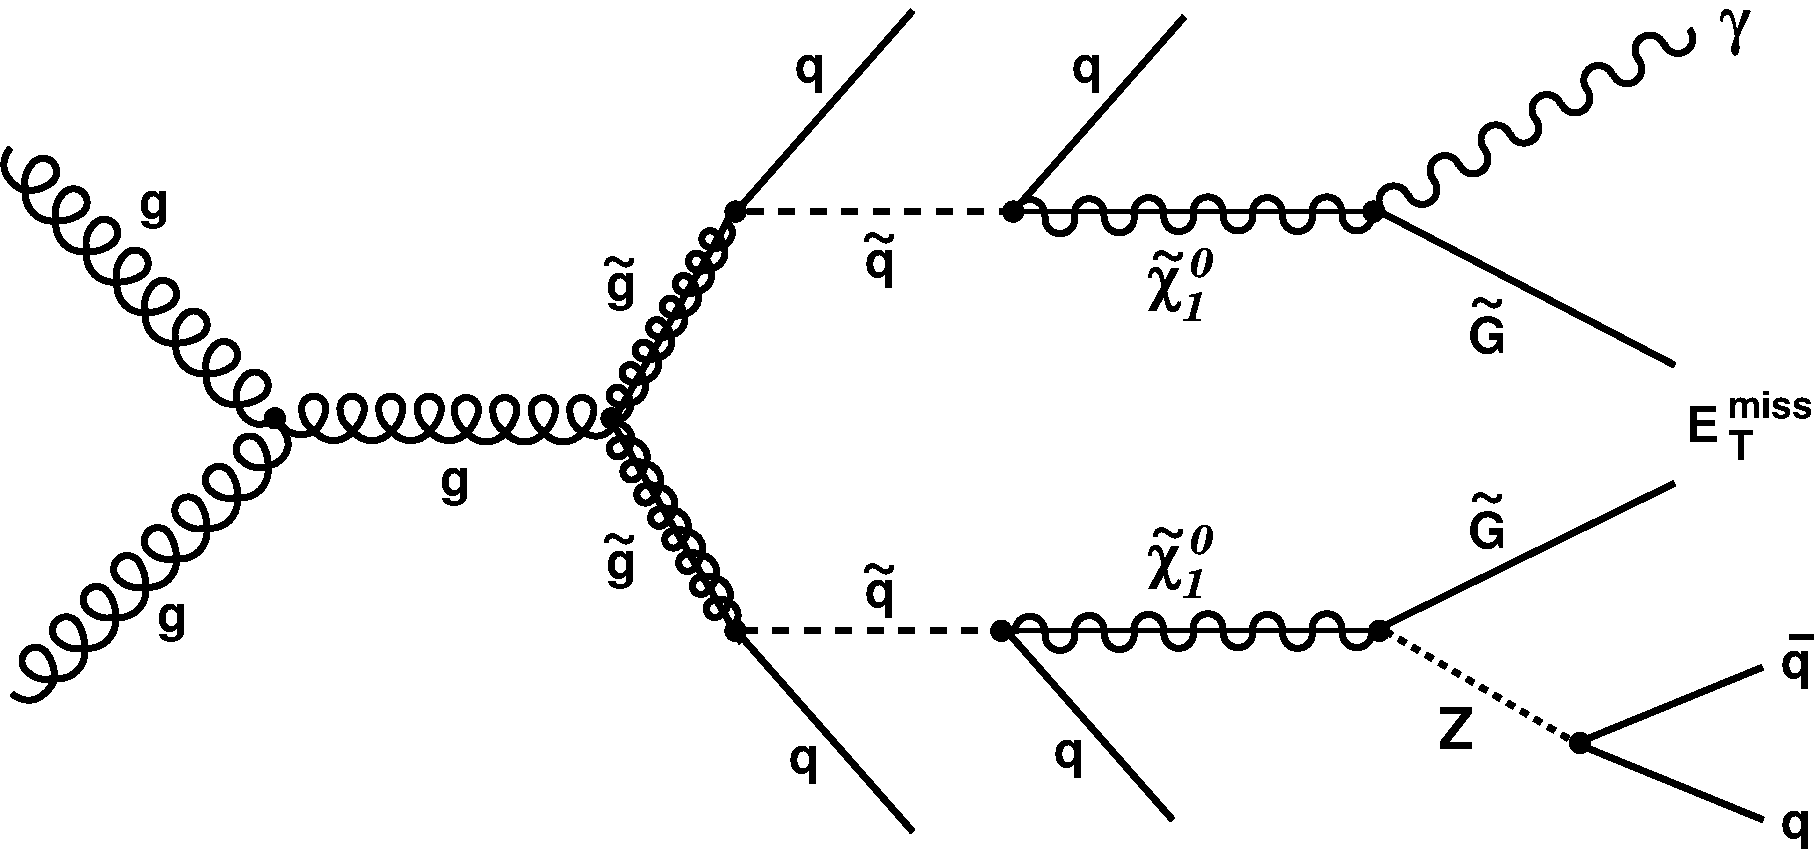
\includegraphics[width=2.5in]{THESISPLOTS/SinglePhoton_gluino.pdf} \quad \quad
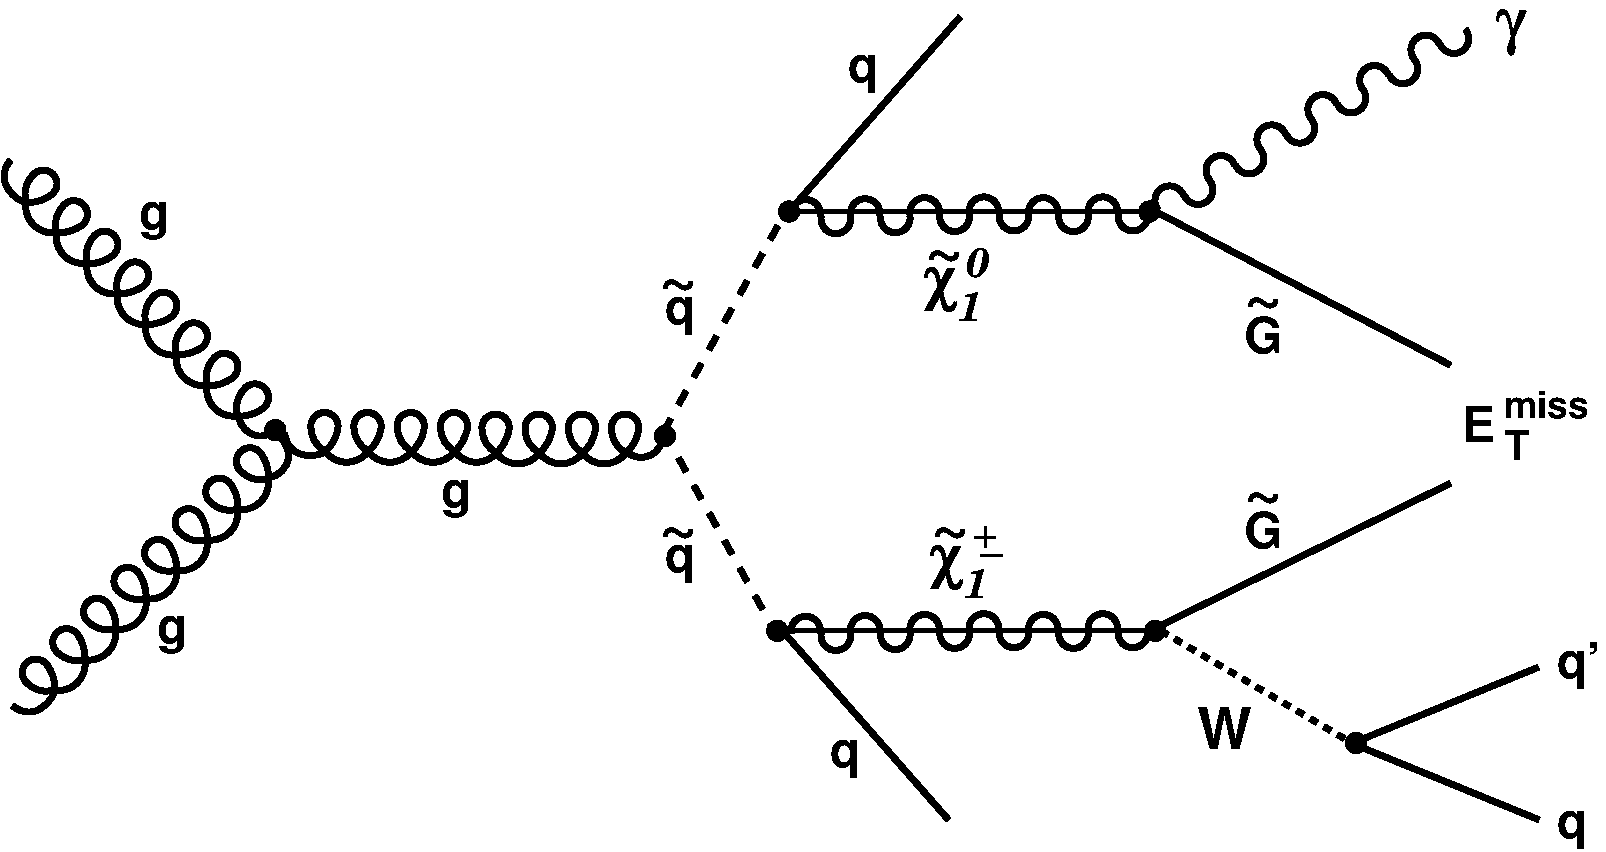
\includegraphics[width=2.5in]{THESISPLOTS/SinglePhoton_squark.pdf}}
\captionof{figure}{Feynman diagrams of of Gravitino interactions with superpartner pairs $(\psi, \phi)$ (a) and $(\lambda, \mathrm{A})$(b).}
\label{fig:feynman_grav}
\end{center}

The presence of light gravitinos allows for the decay of any next-to-lightest MSSM particle to a gravitino as $\tilde{p}\rightarrow p\tilde{G}$ with the decay rate depending on the mass of the gravitino $m_{\tilde{G}}$ as long as R-parity is conserved. Thus  every MSSM particle decay will eventually include a gravitino in its final states. This decay rate can be parametrised by $C_{grav}$. It is easy to see that $C_{grav} \geq 1$.
Thus we define the parameter space for GMSB models as follows:
\begin{itemize}
\item For minimal GMSB~(mGMSB): the parameter space is 
\begin{equation}\label{mGMSB}
\left\{ \Lambda, \quad \mathrm{M}_{\mbox{mess}},\quad \mathrm{N_{5}}, \quad \tan\beta, \quad sgn(\mu),\quad C_{grav}\right\}
 \end{equation}
 
 \item For General Gauge Mediation SUSY breaking~(GGM): The parameter space to scan is  \cite{PMeade,PMeade1}
 \begin{equation}\label{GGM}
 \left\{\mathbf{M_{3}}(\mbox{gluino mass}), \quad \mathbf{M_{2}}(\mbox{Wino mass}), \quad \mathbf{M_{1}}(\mbox{Bino mass}), \quad \tan\beta, \quad sgn(\mu),\quad c\tau_{NLSP}\right\}
 \end{equation}
The advantage with GGM models is that colored sparticles are not required to be be heavier than their electroweak sparticles allowing for greater discovery potential at hadron collider\cite{DSHIH}
\item For Pure General Gauge Mediation SUSY breaking~(PGGM): The parameter space to scan is:
\begin{equation}\label{PGGM}
\left\{\Lambda_{G},\quad \Lambda_{S}, \quad \mathrm{M}_{\mbox{mess}}\right\}
 \end{equation}
 
\end{itemize}

In these models, the Next-To-Lightest SUSY particle~(NLSP) decays to the lightest SUSY particle~(LSP), the gravitino and its SM partner. if $\tilde{p}$ is the NLSP, then it will decay is as follows:
\begin{equation}
\tilde{p}\rightarrow p + \tilde{G}
\end{equation}
In mGMSB models $\tilde{p}$ is the lightest neutralino(neutralinos come in four types and they are a mixture of Bino~($\tilde{B}^{\circ}$),Wino~($\tilde{W}^{\circ}$),
higgsino~($\tilde{H}^{\circ}_{u},\tilde{H}^{\circ}_{d}$) depending on the choice of parameters $M_{1},M_{2},M_{3}$, or $\Lambda$, $\tan\beta$, and $sgn(\mu)$.
and particle $p$ is the photon~($\gamma$),  SM(or new) Z boson)~$(Z)$(or $Z^{\prime}$) and the higgs~($h$).
In this thesis, we will only focus on the parameter space for which the the particle $p = \gamma$ and $C_{grav} > 1$.
This ensures that with the lifetime of our NLSP being finite, its decay happens \textit{within the detector volume} and the resulting photon is delayed or non-prompt on detector time scales.

The decay rate for an NLSP to its SM partner and a gravitino goes like( details can be found in\cite{SM,GU}):
\begin{equation}\label{drate}
\Gamma(\tilde{NLSP} \rightarrow \gamma\tilde{G}) \approx  \frac{m^{5}_{\tilde{NLSP}}}{\mathbf{F}^{4}}
\end{equation}
This approximation is almost the same for the non-minimal GMSB models except that we add other parameters showing explicit dependence of how the neutralino life time can be made as long as expected in collider detectors.
It is important to observe here that, the decay rate is large for smaller values of fundamental SUSY breaking scale or equivalently smaller gravitino mass provided the neutralino mass is kept fixed. Thus if $m_{NLSP}$ is of the $\mathrm{O}(100$~\GeV) or more and $\mathbf{F} \ll 1000$~TeV, meaning $m_{\tilde{G}} \leq 1$~KeV, then the above decay rate is of the order than can be observed at hadron collider detectors.



%%%%%%%%%%%%%%%%%%%%%%%%%%%%%%%%%%%%%%%

%%%%%%%%%%%%%%%%%%%%%%%%%%%%%%%%%%%%%%%%
\section{Long-Lived Particles in GMSB}
\paragraph*{}
We have in previous discussions mentioned in passing some reasons why the study of LL particles is very important for uncovering new physics beyond the SM. In addition to mass, charge and spin being experimental handles for the search of new physics, a particle's life time or decay length is indispensable as importable parameters related to the underlying interaction type of the decay can be extracted from the decay rate and hence provide direct window towards new physics interactions beyond the SM.
\subsection{Production and Decay of Supersymmetric Particles at Hadron Colliders}
%%%%%%%%%%%%%%%%%%%%%%%%%%%%%%%%%%%%%%
\begin{center}
\centering
\mbox{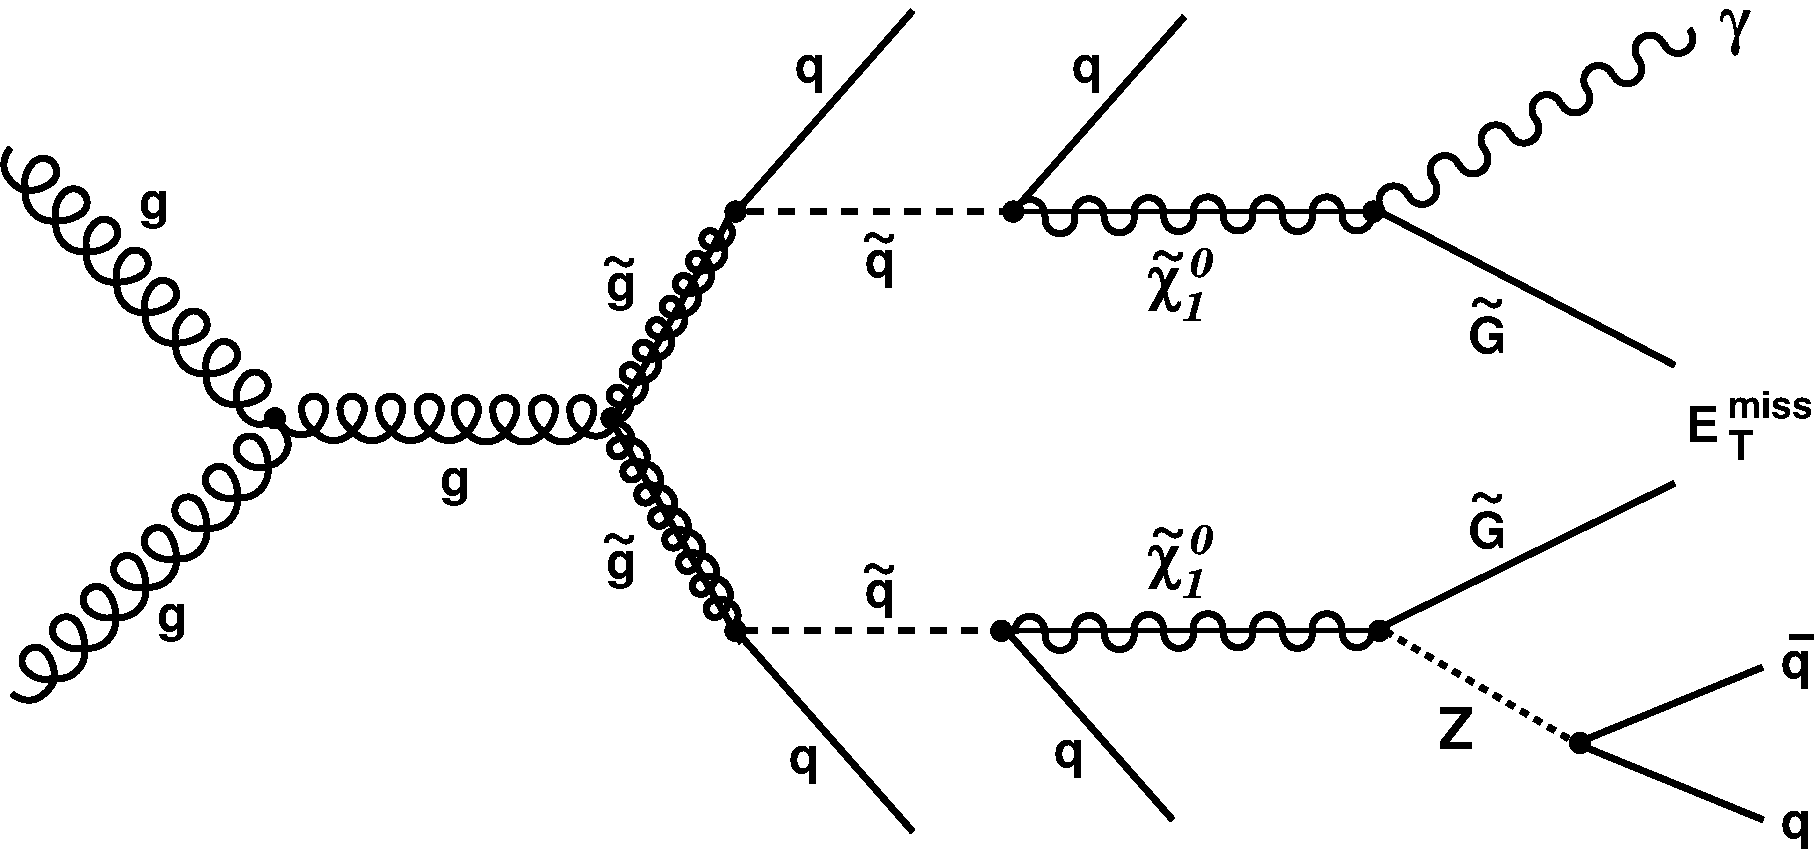
\includegraphics[width=2.5in]{THESISPLOTS/SinglePhoton_gluino.pdf} \quad \quad
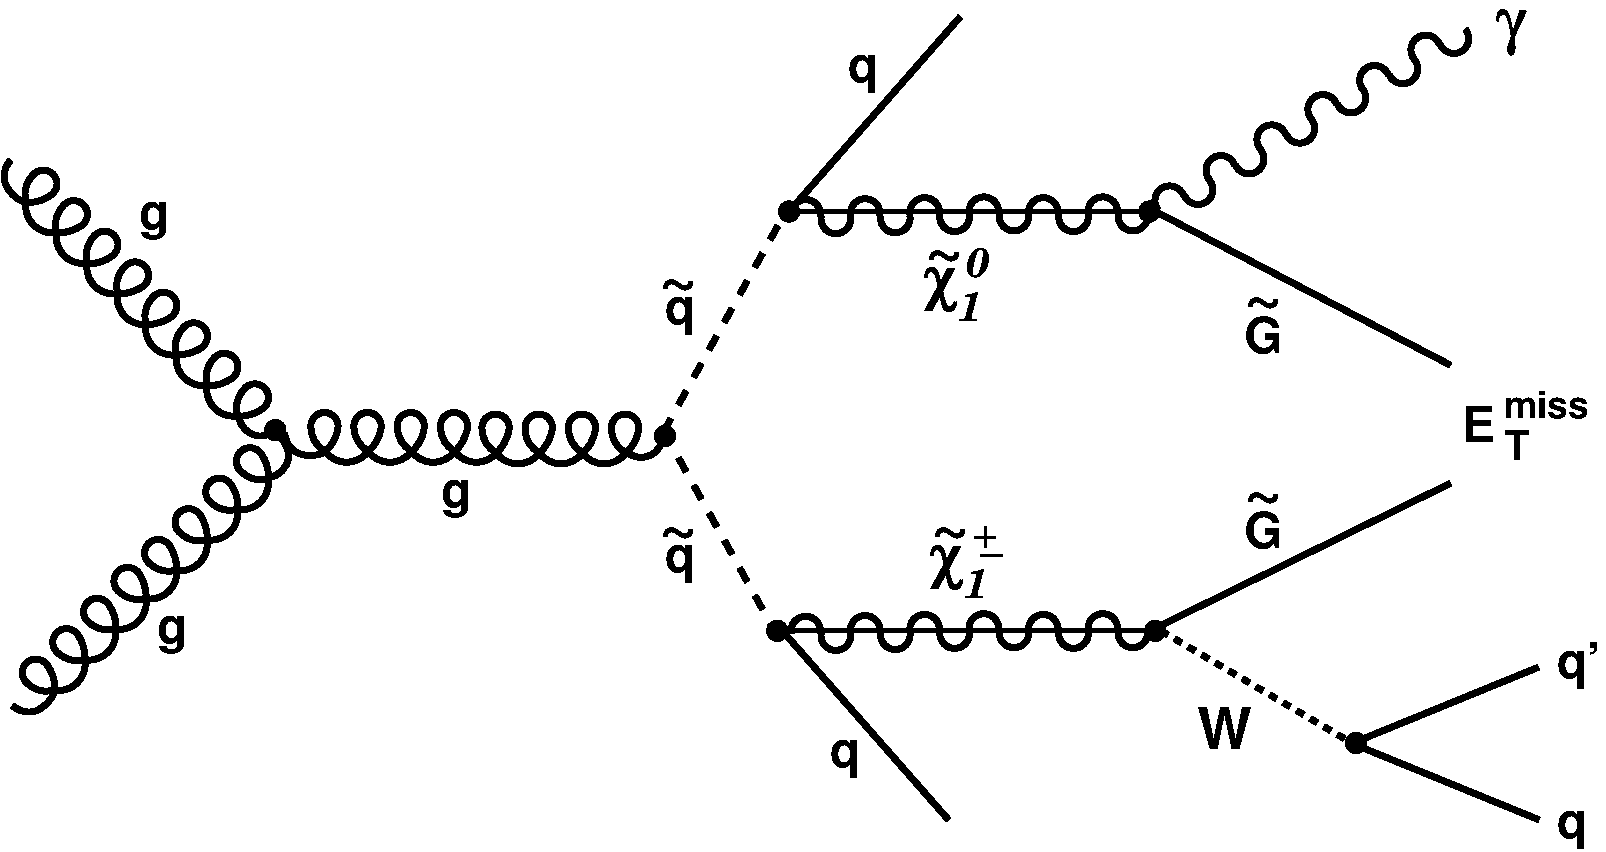
\includegraphics[width=2.5in]{THESISPLOTS/SinglePhoton_squark.pdf}} \\
\hspace{0.5cm}
\mbox{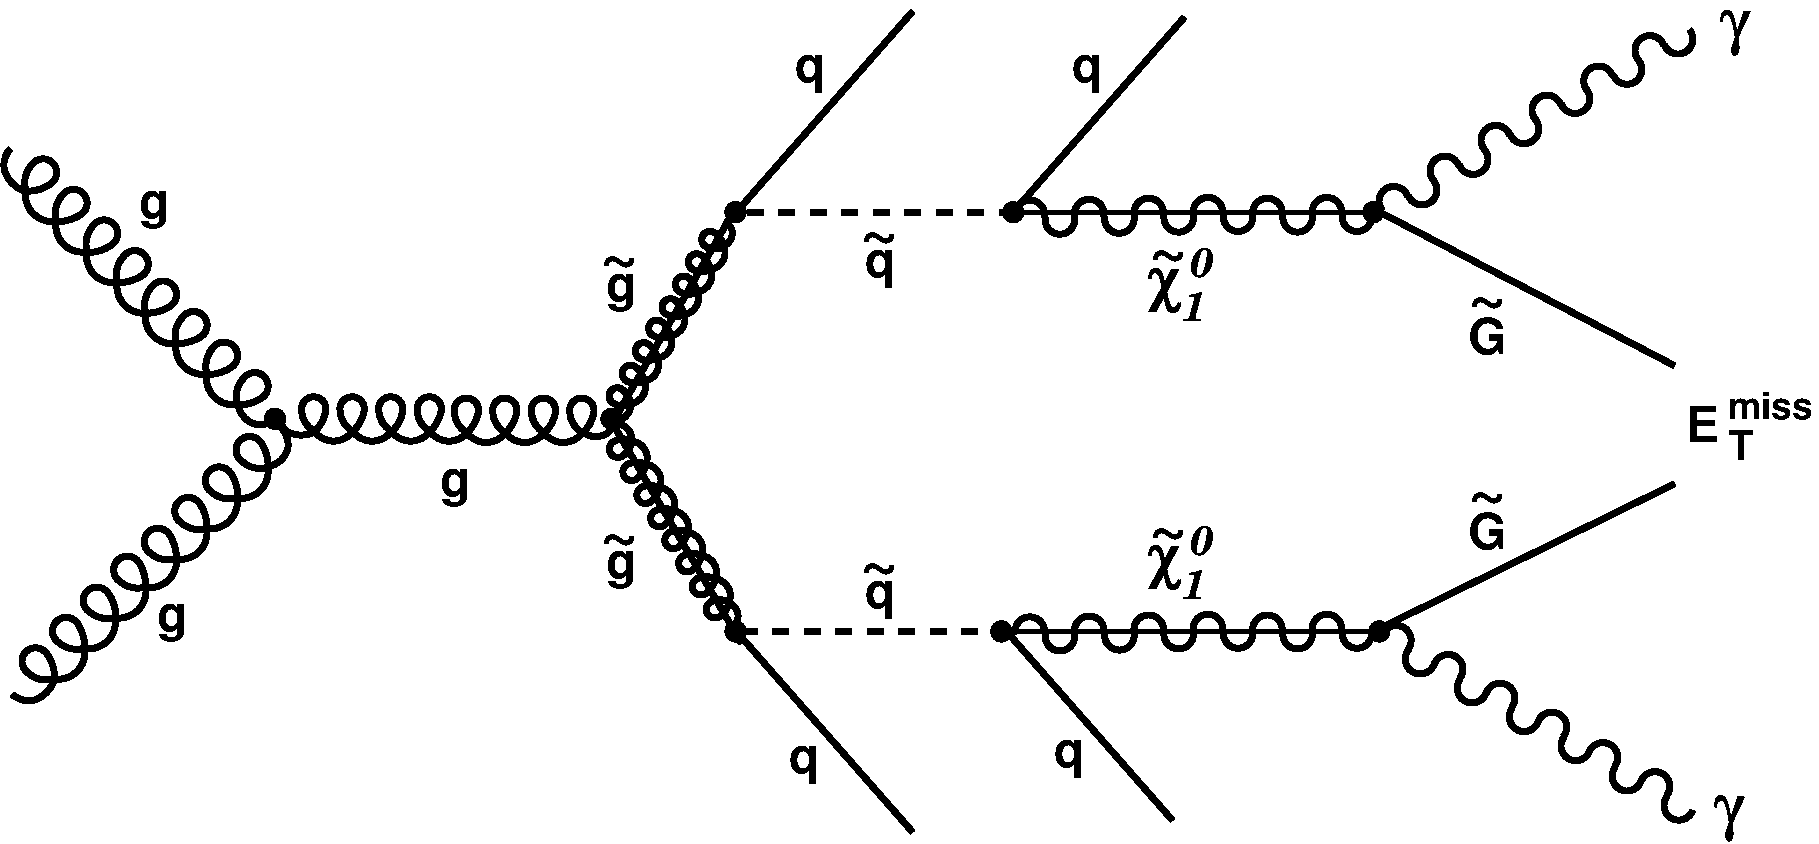
\includegraphics[width=2.5in]{THESISPLOTS/Diphoton_gluino.pdf} \quad \quad
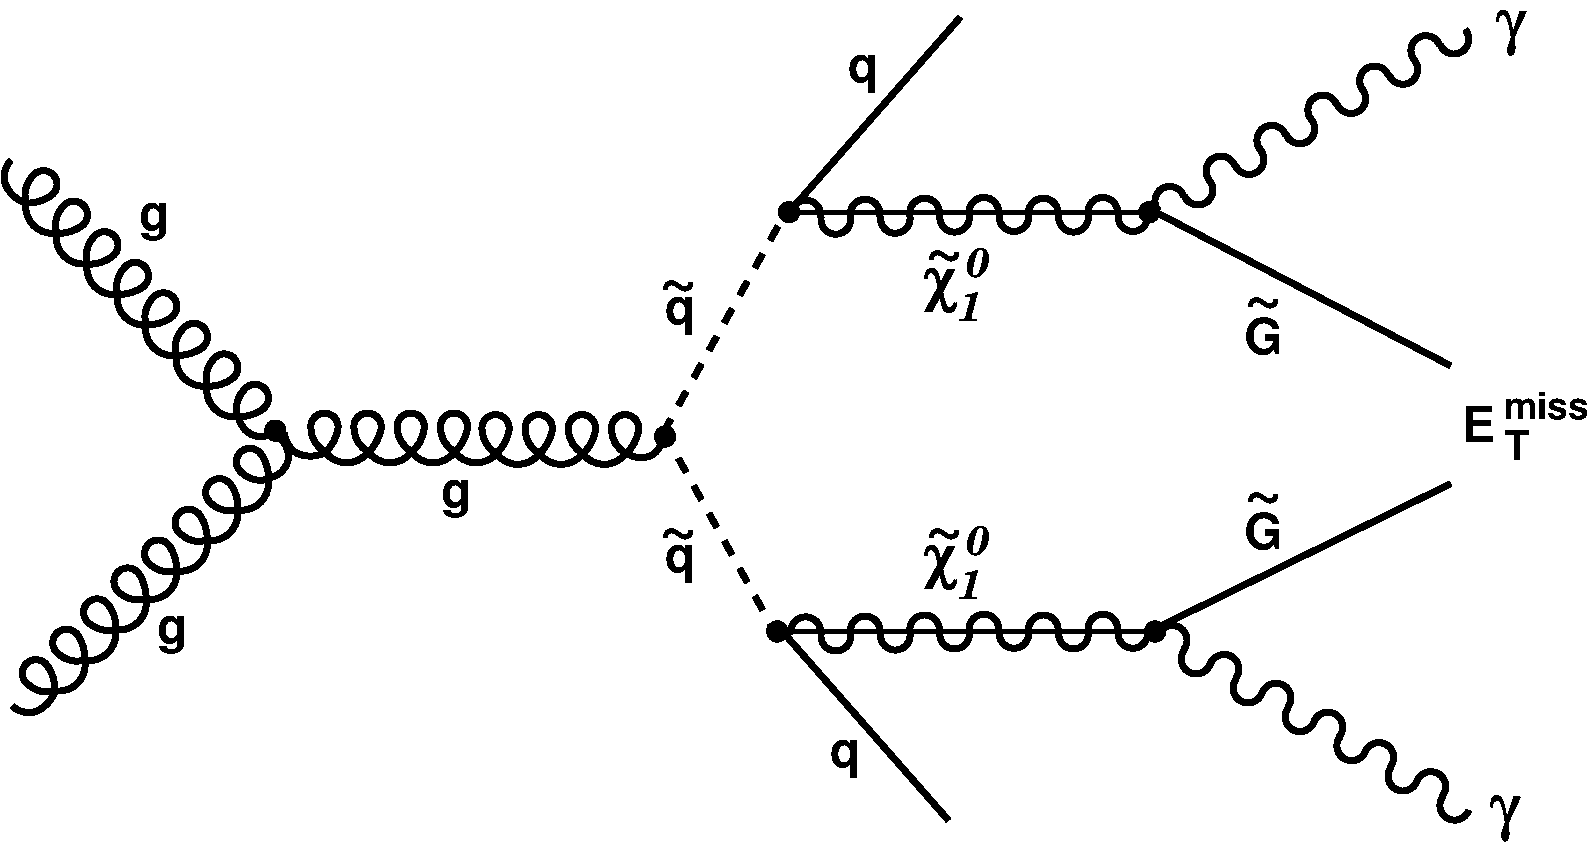
\includegraphics[width=2.5in]{THESISPLOTS/Diphoton_squark.pdf}}
\captionof{figure}{Feynman diagrams of single(top) and di(bottom) photon production from cascade decays of gluino and squark at LHC.}
\label{fig:feynman_gsDiag}
\end{center}

\paragraph{NLSP Decay Length}
\paragraph*{}
The probability for a NLSP particle produced with an energy $\displaystyle{\mathrm{E}}$ having mass $m$ to travel a distance $x$ before decaying to a photon and gravitino in the laboratory frame is given as:
\begin{equation}\label{prop}
\displaystyle{\mathcal{P}(\mathsf{x}) = 1 - \exp{\left(- \frac{x}{\mathrm{L}} \right)} }
\end{equation}
where
\begin{equation}\label{dl}
\displaystyle{\mathrm{L} = c\tau_{NLSP}\cdot\left(\beta\gamma\right)_{NLSP} [mm]}
\end{equation}
and
\begin{equation}\label{ctau}
\displaystyle{\left(\beta\gamma\right) = \frac{|p|}{m} = \sqrt{\left(\frac{E}{m}\right)^{2} - 1} }
\end{equation}
with its proper decay length as given by as(we have used equation 2.23 and \label{drate} 2.64 to go from decay rate to lifetime):
\begin{equation}\label{DRate}
c\tau_{NLSP} \approx \left(\frac{m_{NLSP}}{\mbox{ GeV}}\right)^{-5}\left(\frac{\sqrt{\mathbf{F}}}{\mbox{TeV}}\right)^{4}
\end{equation}
Its is important to observe here that, varying $\mathbf{F}$ changes the lifetime of the NLSP from being prompt to long-lived.
This variation can be easily archived in GMSB models where the parameter $C_{grav}$ is used so that the above proper decay length equation becomes:
\begin{equation}\label{pdlength}
c\tau_{NLSP} \approx C^{2}_{grav} \left(\frac{m_{NLSP}}{\mbox{GeV}}\right)^{-5}\left(\frac{\sqrt{\mathbf{F}_{S}}}{\mbox{TeV}}\right)^{4}
\end{equation}

With $C_{grav}$, one could  one could change the decay length of the NLSP such that its decay occurs within the volume of the detector such that the resulting photon is delayed. This gives a unique signature for discovering SUSY in hadron colliders as photons produced from SM interactions are prompt.
In a simple GMSB model such as the SPS8, where the neutralino is the NLSP and gravitino is LSP, figure \eqref{NKINE} show the kinematic properties and neutralino proper decay length distribution for the neutralino and its decayed photon in different  parameter choices. The HepMC class in CMS Software~(CMSSW) is used to measure and and exponential distribution as the one in \eqref{prop} is fitted on the decay length distribution to extract its proper decay length as produced in the MC generation.
\begin{center}
\centering
\mbox{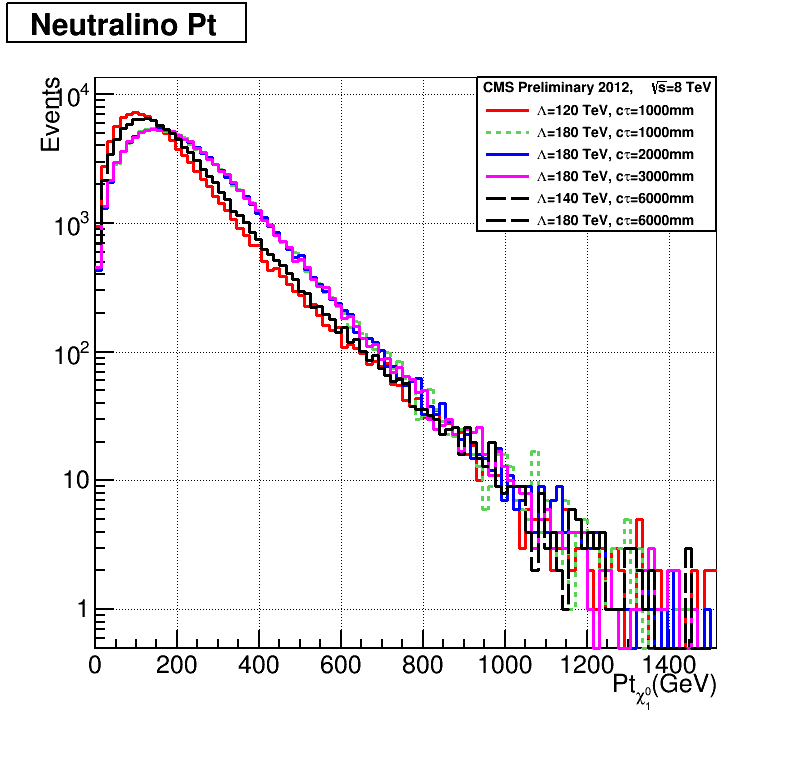
\includegraphics[scale=0.3]{THESISPLOTS/GMSB-SPS8-MODEL-Neutralinio-Pt.png} \hspace{-1cm}
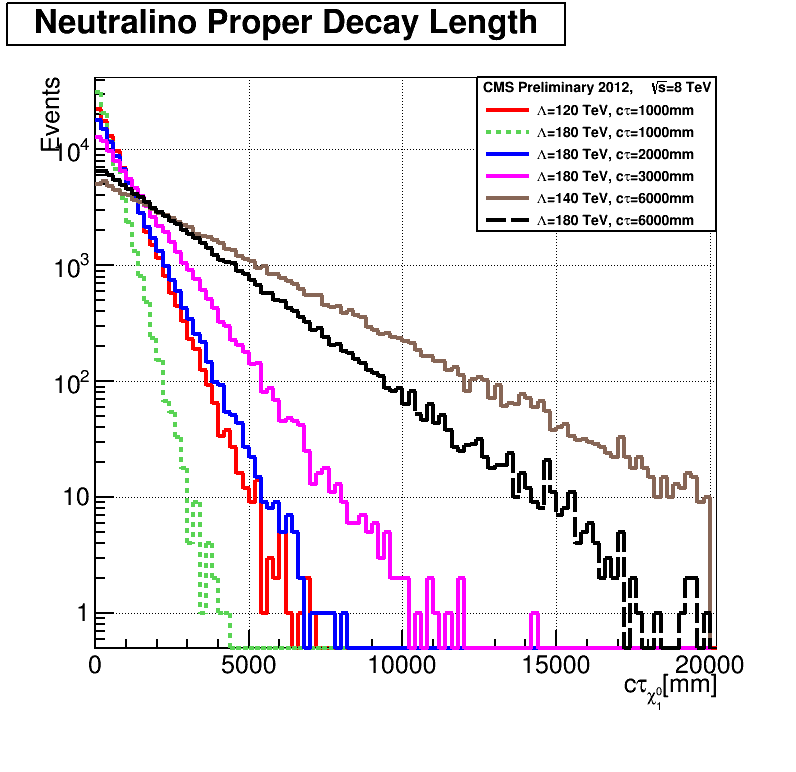
\includegraphics[scale=0.3]{THESISPLOTS/GMSB-SPS8-MODEL-Neutralino-Proper-DecayLength.png}} \\
\hspace{0.5cm}
\mbox{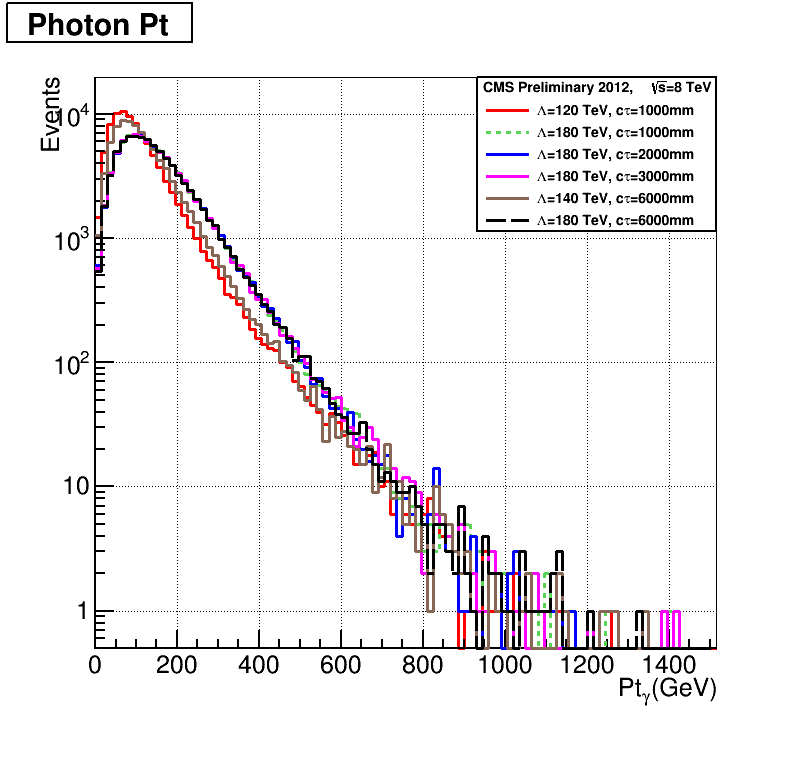
\includegraphics[scale=0.3]{THESISPLOTS/GMSB-SPS8-MODEL-Photon-Pt.png} \hspace{-1cm}
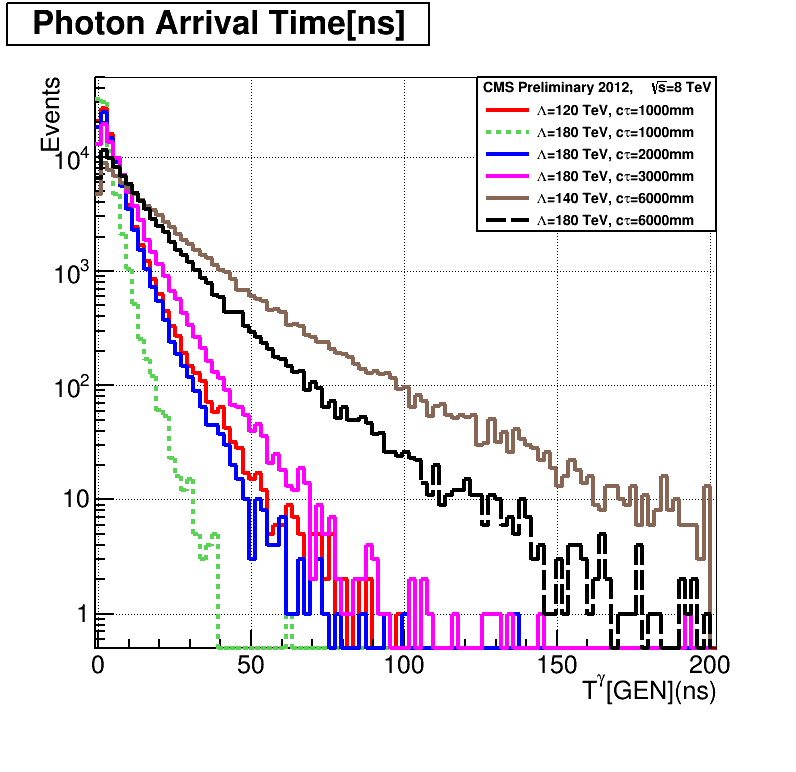
\includegraphics[scale=0.3]{THESISPLOTS/GMSB-SPS8-MODEL-Photon-Arrival-Time.png}}
\captionof{figure}{Neutralino transverse momentum distribution(top left) and proper decay length(top right) with its  decayed photon transverse momentum distribution( Bottom right) and time of arrival at ECAL(Bottom right) for GMSB SPS8 model.}
\label{fig:NKINE}
\end{center}


%\begin{equation}\label{DRate}
%c\tau_{NLSP} = 9.9 \times 10^{-8}\frac{1}{k_{1\gamma}}\left(\frac{m_{NLSP}}{100 GeV}\right)^{-5}\left(\frac{\sqrt{\mathrm{F}}}{10TeV}\right)^{4}
%\end{equation}

%%%%%%%%%%%%%%%%%%%%%%%%%%%%%%%%%%%%%%
\subsection{Advantages in Search for Long-Lived Particles}
\paragraph*{}
 Finding answers to fundamental questions such as the following: What is the origin of neutrino masses, Why are there only 3 types of leptons and quarks? Where do all the parameters in SM come from? Other big questions include: What is Dark Matter ~(DM)? is DM made of particles? Can one detect these particles? Why is there so much asymmetry between matter and anti-matter in our universe? Is there some energy scale or early epoch in the evolution of the universe where all the fundamental forces behaved as a unique kind of force. Do baryons such as the proton exist forever? What is the lifetime of the proton? What is Dark Energy~(DE)? Is the Universe expanding indefinitely? Are there other Universes? 
 provide added impetus to search for particles BSM. We believe that the discovery of a long-live particle which are not known to exist within the current SM will provide unique access to understanding physics BSM and making measurements which can provide answers to most of the above questions.
\newline{}
%These questions have been addressed in two major fronts: Theoretically which involves lots of model building and Experimentally which can be divided into Observational as well as Collider Experiments. Most of these experiments involves the search for w new physics phenomenon. In this Thesis, we have decided to address some of these questions by searching for New Physics phenomenon or New Particles ~(NP) in a Hadron Collider experiment. 
%As a consequence, there are many searches for New Particles or New Physics~(NP) 
Searching for LL neutral particles decaying to photon using timing gives us a unique advantage compared to other experiments as we expect very limited background process contribution from SM. Most of our background will be detector originated contributions
%Infact, we are searching for some NP which have been predicted to exist in nature by many Theoretical extensions of the SM collectively referred to as Beyond the Standard Model~(BSM). We will describe one of such models in the next section below.
%We are interested in searching for neutral NP through their lifetime. 
Infact, our search using lifetime gives us a wide range of search techniques  depending on the lifetime of the LL particle ranging from quantitative measurements to statistics. The figure below  shows the wide variety of techniques which can be used to search for LL particles in general.
\begin{equation}
\mbox{ADD figure of techniques for Searches using LL}
\end{equation}
%\begin{figure}
%\centering
%\includegraphics[scale=0.5]{}
%\caption{Different techniques to Search for LL particles.}
%\end{figure}
Using equations \eqref{ctau}, precise measurement of fundamental parameters in SUSY or new physics can be archived.
Another advantage is that, the our search for neutral particles  is unique in that a lot of previous searches been performed for charged particles but very limited for neutral LL particles since DM is speculated to be made of stable neutral particle(s) with long lifetime, we might as well go for DM. 
We also use lifetime because no particle with lifetime $\gtrsim10^{-7}$~s and mass $\gtrsim 1.5$~GeV has been found and obviously because our detector has a very good timing resolution as can be seen in the section of the CMS detector in this thesis.
\newline{}
There have been previous attempts to search for quasi-stable neutral massive particles but all the search results show no evidence for neutral particles with long lifetime.  
%or neutral particles in general or neutral hadrons in particular 
The challenge with such an experiment is that neutral particles cannot be studied using conventional magnetic spectrometer as they are not affected by magnetic field because they are charge~(local 
U(1) gauge symmetry) neutral.
Nevertheless, there are countless theoretical as well as observational reasons why studying these particles using novel experimental techniques is very important in the field of particle physics. 
Some of these reasons will emerge naturally as we see in the subsequent sections below.
%We will attempt to give our humble lists of reasons in the following
%sections why we believe it is fundamental to study these particles.
\subsubsection{Motivation from Theory.}
Physics BSM can be summarized to answering three major theoretical questions:  Is there a reliable explanation  
behind the ordering in mass of SM particles as observed? This is the Hierarchy problem.
Is there a single theory which can provide a derivation for all the 
numerous parameters (19) in the SM and also unify all the fundamental forces of nature? Grand Unified Theories (GUT). 
What is DM and Dark Energy (DE)?
(DE is the stuff that is responsible for the accelerated expansion of our universe).
And finally being a particle physicist it is only natural to ask if DM is made up of particles and if yes,
Can one construct a model which can consistently describe DM as is already the case with visible matter in SM?
\newline
Most of the efforts in the last decades in theoretical particle physics has been to find answers to the above questions.
\subsubsection{Motivation From Experiment and Observation}
As early as 1956 Reines and Cowan\cite{Neutrino} observed that when a neutron decays into a proton and an electron, an elusive particle called neutrino is also produced. The observation of neutrinos was later incorporated into the SM. In the formulation of the SM, the neutrinos are considered massless.
However, recent results from experiments \cite{NeutrinoMix} have shown that neutrinos of different flavours can oscillate or mix into one another. The only way they can do this is if they have a tiny but finite mass. Recent experiments measuring the different neutrino flavours and their mass difference point towards the existence of a much larger theory that can incorporate the existence of neutrino masses and the observed phenomenon of neutrino mixing in which the SM is embedded in it   and can be understood as a low energy version of a much broader and deeper theory.
\paragraph*{}
Galactic and supernovae observations using the Hubble and a host of other telescope as well as results from Baryonic Acoustic Oscillation~(BAO) and WMAP reveal unique matter content of our universe. In addition to these cosmological observations including galaxy profiles,cluster formation, large scale structure formation and Cosmic Microwave background~(CMB) power spectrum can be somehow explained by DM \cite{WMAP}. These observation reveals about 25\% of our universe is made of DM with the current DM relic density is measured to be  %${\POmega}_{DM}h^{2} = {0.105} ^{\p 0.021}_{\m 0.030}$
However, the question of "What is DM?" remains a very interesting one to both the particle physics astronomy society.
Understanding DM and the rest of our universe will be crucial for future developments in high energy physics from both theory and experimental fronts.  
A possible property of DM is that they must be made of up long lived neutral particles. There are candidate particles from SUSY which have these properties. A few of these include lightest neutralino~(\PSneutralinoOne) and gravitino~($\tilde{G}$). From the GMSB point of view, because gravitinos are stable, neutral and very weakly interacting; they are seen as good candidates for the particles which make up DM. 
%\subsubsection{Current Experimental Limits}
%Past Experiments seems to indicate that the remaining un %searched phase space for possible existence of SUSY particles %in shrinking.
%%%%%%%%%%%%%%%%%%%%%%%%%%%%%%%%%%%%%%%%%%%%
%%%%%%%%%%%%%%%%%%%%%%%%%%%%%%%%%%%%%%%%%
%\subsection{Physics}
%\paragraph*{}
% The SM of particle physics in all its glory is the most precise and well developed model describing and providing our understanding of how energy, space and time interact with each other. We will begin by describing the current status of the SM highlighting areas where there could be need for further development in the format of questions.
%%%%%%%%%%%%%%%%%%%%%%%%%%%%%%%%%%%%%%%%%%%%%%%%%%%%%%%%%%%%%%%%%%%%%%%%%%%%%%%%
%%%%%%%%%%%%%%%%%%%%%%%%%%%%%%%%%%%%%%%%%%%%%%%%%%%%%%%%%%%%%%%%%%%%%%%%%%%%%%%%
\section{Previous Experiments and Results}
%%%%%%%%%%%%%%%%%%%%%%%%%%%%%%%%%%%%%%%
The hunt for the discovery of DM and new particles, has led to several experimental search  for neutral long-live particles decaying to photons. Obviously, negative results from these experiments has led to the putting limits of the lifetime, mass and cross section of possible existence of SUSY particles in different models of SUSY. Results from experiments(DO, CDF, CMS and ATLAS)\cite{CMS7TeV,ATLAS7TeV} in the search for Neutralino NLSP decaying to photon and gravitino  and interpreted within the Snowmass Point and Slop~(SPS)8 benchmark\cite{SPS8} scenario with parameter set be seen in figures 2.3(a) and (b). These results show that within the SPS8 model, neutralinos with mass $m_{\tilde{\chi}^{0}_{1}} \leq 245$~\GeV and proper decay length $c\tau_{\tilde{\chi}^{0}_{1}} \leq 6000$~mm cannot exist at hadron colliders and thus their existence has been excluded.

%%%%%%%%%%%%%%%%%%%%%%%%%%%%%%%%%%%%%%%
\begin{center}
\centering
\mbox{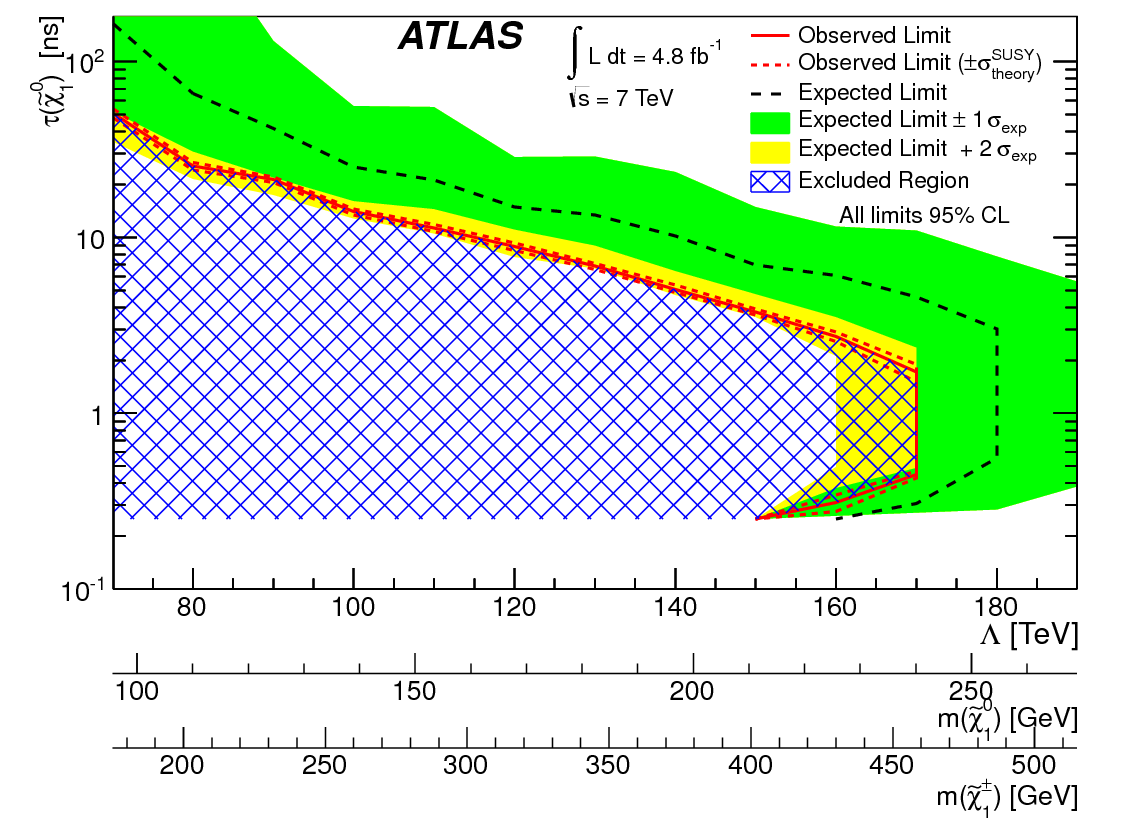
\includegraphics[height=2.4in,width=3.0in]
{THESISPLOTS/ATLAS_Upper_Limit.png} \quad
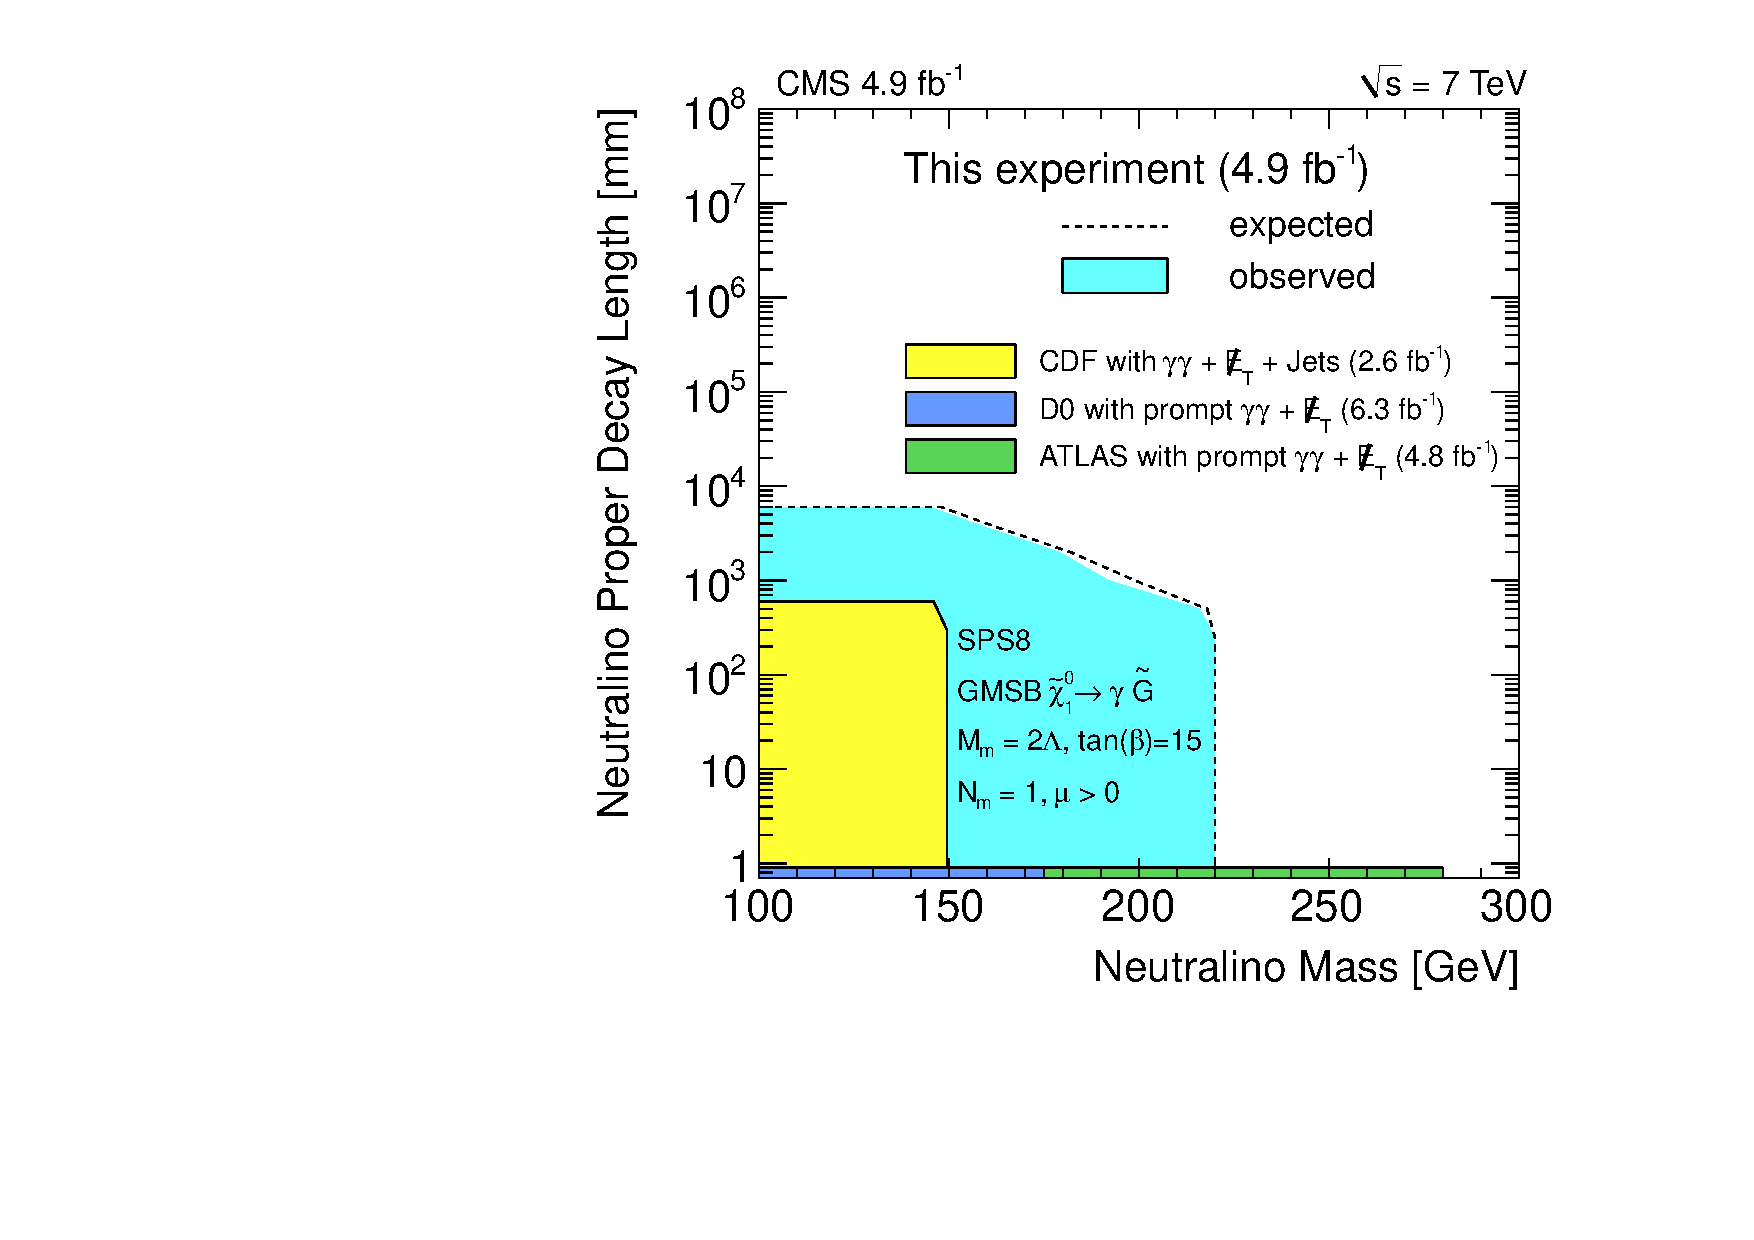
\includegraphics[height=2.5in,width=3.0in]{THESISPLOTS/2D_exclusion.pdf}}
\captionof{figure}{Neutralino lifetime and mass upper limit from ATLAS(left) and CMS(right) 7~TeV analysis with non-pointing photons and MET.}
\label{fig:UpperLimits}
\end{center}